\documentclass[]{article}
\usepackage{lmodern}
\usepackage{amssymb,amsmath}
\usepackage{ifxetex,ifluatex}
\usepackage{fixltx2e} % provides \textsubscript
\ifnum 0\ifxetex 1\fi\ifluatex 1\fi=0 % if pdftex
  \usepackage[T1]{fontenc}
  \usepackage[utf8]{inputenc}
\else % if luatex or xelatex
  \ifxetex
    \usepackage{mathspec}
  \else
    \usepackage{fontspec}
  \fi
  \defaultfontfeatures{Ligatures=TeX,Scale=MatchLowercase}
\fi
% use upquote if available, for straight quotes in verbatim environments
\IfFileExists{upquote.sty}{\usepackage{upquote}}{}
% use microtype if available
\IfFileExists{microtype.sty}{%
\usepackage{microtype}
\UseMicrotypeSet[protrusion]{basicmath} % disable protrusion for tt fonts
}{}
\usepackage[margin=1in]{geometry}
\usepackage{hyperref}
\hypersetup{unicode=true,
            pdftitle={Growth\_mort},
            pdfauthor={Carmen},
            pdfborder={0 0 0},
            breaklinks=true}
\urlstyle{same}  % don't use monospace font for urls
\usepackage{color}
\usepackage{fancyvrb}
\newcommand{\VerbBar}{|}
\newcommand{\VERB}{\Verb[commandchars=\\\{\}]}
\DefineVerbatimEnvironment{Highlighting}{Verbatim}{commandchars=\\\{\}}
% Add ',fontsize=\small' for more characters per line
\usepackage{framed}
\definecolor{shadecolor}{RGB}{248,248,248}
\newenvironment{Shaded}{\begin{snugshade}}{\end{snugshade}}
\newcommand{\KeywordTok}[1]{\textcolor[rgb]{0.13,0.29,0.53}{\textbf{#1}}}
\newcommand{\DataTypeTok}[1]{\textcolor[rgb]{0.13,0.29,0.53}{#1}}
\newcommand{\DecValTok}[1]{\textcolor[rgb]{0.00,0.00,0.81}{#1}}
\newcommand{\BaseNTok}[1]{\textcolor[rgb]{0.00,0.00,0.81}{#1}}
\newcommand{\FloatTok}[1]{\textcolor[rgb]{0.00,0.00,0.81}{#1}}
\newcommand{\ConstantTok}[1]{\textcolor[rgb]{0.00,0.00,0.00}{#1}}
\newcommand{\CharTok}[1]{\textcolor[rgb]{0.31,0.60,0.02}{#1}}
\newcommand{\SpecialCharTok}[1]{\textcolor[rgb]{0.00,0.00,0.00}{#1}}
\newcommand{\StringTok}[1]{\textcolor[rgb]{0.31,0.60,0.02}{#1}}
\newcommand{\VerbatimStringTok}[1]{\textcolor[rgb]{0.31,0.60,0.02}{#1}}
\newcommand{\SpecialStringTok}[1]{\textcolor[rgb]{0.31,0.60,0.02}{#1}}
\newcommand{\ImportTok}[1]{#1}
\newcommand{\CommentTok}[1]{\textcolor[rgb]{0.56,0.35,0.01}{\textit{#1}}}
\newcommand{\DocumentationTok}[1]{\textcolor[rgb]{0.56,0.35,0.01}{\textbf{\textit{#1}}}}
\newcommand{\AnnotationTok}[1]{\textcolor[rgb]{0.56,0.35,0.01}{\textbf{\textit{#1}}}}
\newcommand{\CommentVarTok}[1]{\textcolor[rgb]{0.56,0.35,0.01}{\textbf{\textit{#1}}}}
\newcommand{\OtherTok}[1]{\textcolor[rgb]{0.56,0.35,0.01}{#1}}
\newcommand{\FunctionTok}[1]{\textcolor[rgb]{0.00,0.00,0.00}{#1}}
\newcommand{\VariableTok}[1]{\textcolor[rgb]{0.00,0.00,0.00}{#1}}
\newcommand{\ControlFlowTok}[1]{\textcolor[rgb]{0.13,0.29,0.53}{\textbf{#1}}}
\newcommand{\OperatorTok}[1]{\textcolor[rgb]{0.81,0.36,0.00}{\textbf{#1}}}
\newcommand{\BuiltInTok}[1]{#1}
\newcommand{\ExtensionTok}[1]{#1}
\newcommand{\PreprocessorTok}[1]{\textcolor[rgb]{0.56,0.35,0.01}{\textit{#1}}}
\newcommand{\AttributeTok}[1]{\textcolor[rgb]{0.77,0.63,0.00}{#1}}
\newcommand{\RegionMarkerTok}[1]{#1}
\newcommand{\InformationTok}[1]{\textcolor[rgb]{0.56,0.35,0.01}{\textbf{\textit{#1}}}}
\newcommand{\WarningTok}[1]{\textcolor[rgb]{0.56,0.35,0.01}{\textbf{\textit{#1}}}}
\newcommand{\AlertTok}[1]{\textcolor[rgb]{0.94,0.16,0.16}{#1}}
\newcommand{\ErrorTok}[1]{\textcolor[rgb]{0.64,0.00,0.00}{\textbf{#1}}}
\newcommand{\NormalTok}[1]{#1}
\usepackage{graphicx,grffile}
\makeatletter
\def\maxwidth{\ifdim\Gin@nat@width>\linewidth\linewidth\else\Gin@nat@width\fi}
\def\maxheight{\ifdim\Gin@nat@height>\textheight\textheight\else\Gin@nat@height\fi}
\makeatother
% Scale images if necessary, so that they will not overflow the page
% margins by default, and it is still possible to overwrite the defaults
% using explicit options in \includegraphics[width, height, ...]{}
\setkeys{Gin}{width=\maxwidth,height=\maxheight,keepaspectratio}
\IfFileExists{parskip.sty}{%
\usepackage{parskip}
}{% else
\setlength{\parindent}{0pt}
\setlength{\parskip}{6pt plus 2pt minus 1pt}
}
\setlength{\emergencystretch}{3em}  % prevent overfull lines
\providecommand{\tightlist}{%
  \setlength{\itemsep}{0pt}\setlength{\parskip}{0pt}}
\setcounter{secnumdepth}{0}
% Redefines (sub)paragraphs to behave more like sections
\ifx\paragraph\undefined\else
\let\oldparagraph\paragraph
\renewcommand{\paragraph}[1]{\oldparagraph{#1}\mbox{}}
\fi
\ifx\subparagraph\undefined\else
\let\oldsubparagraph\subparagraph
\renewcommand{\subparagraph}[1]{\oldsubparagraph{#1}\mbox{}}
\fi

%%% Use protect on footnotes to avoid problems with footnotes in titles
\let\rmarkdownfootnote\footnote%
\def\footnote{\protect\rmarkdownfootnote}

%%% Change title format to be more compact
\usepackage{titling}

% Create subtitle command for use in maketitle
\providecommand{\subtitle}[1]{
  \posttitle{
    \begin{center}\large#1\end{center}
    }
}

\setlength{\droptitle}{-2em}

  \title{Growth\_mort}
    \pretitle{\vspace{\droptitle}\centering\huge}
  \posttitle{\par}
    \author{Carmen}
    \preauthor{\centering\large\emph}
  \postauthor{\par}
      \predate{\centering\large\emph}
  \postdate{\par}
    \date{October 31, 2019}


\begin{document}
\maketitle

\section{Next step: Consider adding CEIN to the initialization even
though there isn't any in the American River
footprint}\label{next-step-consider-adding-cein-to-the-initialization-even-though-there-isnt-any-in-the-american-river-footprint}

\section{This script runs simulations with the most up-to-date
functions}\label{this-script-runs-simulations-with-the-most-up-to-date-functions}

\section{Define parameters}\label{define-parameters}

\begin{Shaded}
\begin{Highlighting}[]
\NormalTok{fire <-}\StringTok{ "AMRC"}
\NormalTok{year <-}\StringTok{ "2016"}
\NormalTok{years <-}\StringTok{ }\DecValTok{20}
\NormalTok{iterations <-}\StringTok{ }\DecValTok{1000}
\NormalTok{max_shrub_ht_cm <-}\StringTok{ }\DecValTok{250}
\NormalTok{max_shrub_ht_years <-}\StringTok{ }\DecValTok{15}
\NormalTok{n_seedlings <-}\StringTok{ }\DecValTok{100}
\NormalTok{length_m <-}\StringTok{ }\DecValTok{40}
\NormalTok{height_m <-}\StringTok{ }\DecValTok{40}
\NormalTok{lambda <-}\StringTok{ }\DecValTok{4}
\NormalTok{shrub_clumpiness <-}\StringTok{ }\DecValTok{7}
\end{Highlighting}
\end{Shaded}

\section{Load functions}\label{load-functions}

\paragraph{Create shrub patch}\label{create-shrub-patch}

\begin{Shaded}
\begin{Highlighting}[]
\KeywordTok{source}\NormalTok{(}\StringTok{"functions/shrubclump.R"}\NormalTok{)}
\end{Highlighting}
\end{Shaded}

\paragraph{Initialization function}\label{initialization-function}

\begin{Shaded}
\begin{Highlighting}[]
\KeywordTok{source}\NormalTok{(}\StringTok{"functions/initialize.R"}\NormalTok{)}
\end{Highlighting}
\end{Shaded}

\paragraph{Height growth functions}\label{height-growth-functions}

\begin{Shaded}
\begin{Highlighting}[]
\KeywordTok{source}\NormalTok{(}\StringTok{"functions/abcogrowth.R"}\NormalTok{)}
\KeywordTok{source}\NormalTok{(}\StringTok{"functions/pipogrowth.R"}\NormalTok{)}
\end{Highlighting}
\end{Shaded}

\paragraph{Diameter growth functions}\label{diameter-growth-functions}

\begin{Shaded}
\begin{Highlighting}[]
\KeywordTok{source}\NormalTok{(}\StringTok{"functions/abcodia.R"}\NormalTok{)}
\KeywordTok{source}\NormalTok{(}\StringTok{"functions/pipodia.R"}\NormalTok{)}
\end{Highlighting}
\end{Shaded}

\paragraph{Mortality functions}\label{mortality-functions}

\begin{Shaded}
\begin{Highlighting}[]
\KeywordTok{source}\NormalTok{(}\StringTok{"functions/abcomort.R"}\NormalTok{)}
\KeywordTok{source}\NormalTok{(}\StringTok{"functions/pipomort.R"}\NormalTok{)}
\end{Highlighting}
\end{Shaded}

\paragraph{Shrub growth functions}\label{shrub-growth-functions}

\begin{Shaded}
\begin{Highlighting}[]
\KeywordTok{source}\NormalTok{(}\StringTok{"functions/abco_shrubgrowth.R"}\NormalTok{)}
\KeywordTok{source}\NormalTok{(}\StringTok{"functions/pipo_shrubgrowth.R"}\NormalTok{)}
\end{Highlighting}
\end{Shaded}

\paragraph{Simulation function}\label{simulation-function}

\begin{Shaded}
\begin{Highlighting}[]
\KeywordTok{source}\NormalTok{(}\StringTok{"functions/sim.R"}\NormalTok{)}
\end{Highlighting}
\end{Shaded}

\paragraph{Iteration function}\label{iteration-function}

\begin{Shaded}
\begin{Highlighting}[]
\KeywordTok{source}\NormalTok{(}\StringTok{"functions/iterate.R"}\NormalTok{)}
\end{Highlighting}
\end{Shaded}

\section{Initialize}\label{initialize}

\subsection{Create clumped shrub
pattern}\label{create-clumped-shrub-pattern}

\begin{Shaded}
\begin{Highlighting}[]
\KeywordTok{shrubclump}\NormalTok{()}
\KeywordTok{plot}\NormalTok{(r)}
\end{Highlighting}
\end{Shaded}

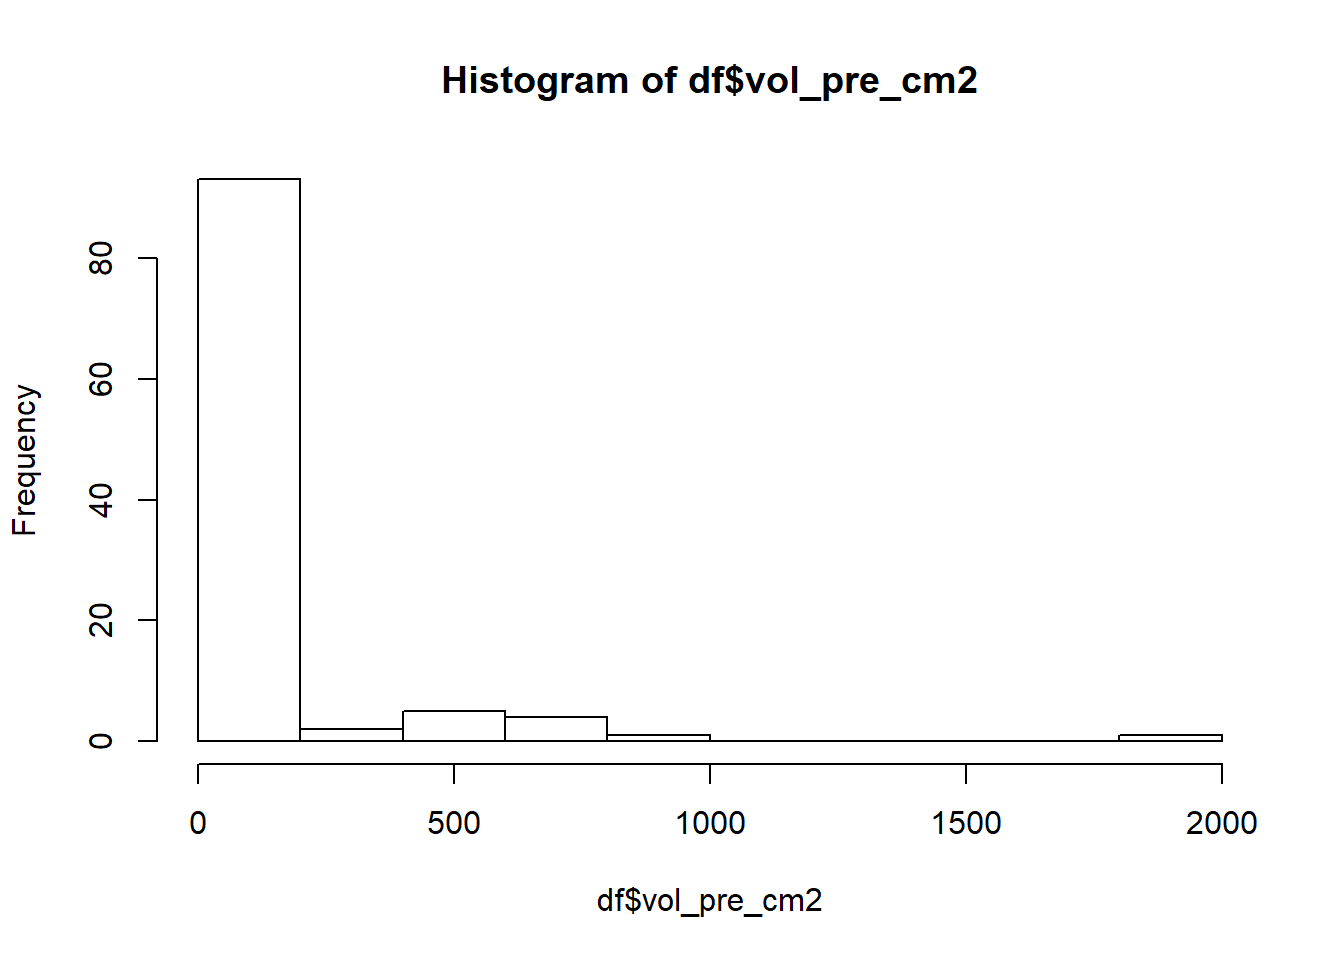
\includegraphics{simulations_files/figure-latex/unnamed-chunk-11-1.pdf}

\subsection{Randomly select seedlings from data and place them on the
shrub
patch}\label{randomly-select-seedlings-from-data-and-place-them-on-the-shrub-patch}

\begin{Shaded}
\begin{Highlighting}[]
\KeywordTok{initialize}\NormalTok{()}
\end{Highlighting}
\end{Shaded}

\begin{verbatim}
## Joining, by = "ID"
\end{verbatim}

\begin{verbatim}
## Joining, by = "Sdlg"
\end{verbatim}

\begin{verbatim}
## Warning: Column `Sdlg` joining factors with different levels, coercing to
## character vector
\end{verbatim}

\subsection{Plot patch with seedlings}\label{plot-patch-with-seedlings}

\begin{Shaded}
\begin{Highlighting}[]
\NormalTok{max_shrub <-}\StringTok{ }\KeywordTok{max}\NormalTok{(r}\OperatorTok{@}\NormalTok{data}\OperatorTok{@}\NormalTok{attributes[[}\DecValTok{1}\NormalTok{]]}\OperatorTok{$}\NormalTok{sqrt_shrubarea3)}
\NormalTok{r}\OperatorTok{@}\NormalTok{data}\OperatorTok{@}\NormalTok{attributes[[}\DecValTok{1}\NormalTok{]]}\OperatorTok{$}\NormalTok{shrub_rel <-}\StringTok{ }\NormalTok{r}\OperatorTok{@}\NormalTok{data}\OperatorTok{@}\NormalTok{attributes[[}\DecValTok{1}\NormalTok{]]}\OperatorTok{$}\NormalTok{sqrt_shrubarea3}\OperatorTok{/}\NormalTok{max_shrub}
\end{Highlighting}
\end{Shaded}

\begin{Shaded}
\begin{Highlighting}[]
\NormalTok{pts.sf.pipo.graph <-}\StringTok{ }\NormalTok{pts.sf.pipo }\OperatorTok\StringTok{ }
\StringTok{  }\KeywordTok{rename}\NormalTok{(}\StringTok{"Pine height"}\NormalTok{ =}\StringTok{ }\NormalTok{Ht_cm1)}
\NormalTok{pts.sf.abco.graph <-}\StringTok{ }\NormalTok{pts.sf.abco }\OperatorTok\StringTok{ }
\StringTok{  }\KeywordTok{rename}\NormalTok{(}\StringTok{"Fir height"}\NormalTok{ =}\StringTok{ }\NormalTok{Ht_cm1)}
\end{Highlighting}
\end{Shaded}

\begin{Shaded}
\begin{Highlighting}[]
\KeywordTok{tm_shape}\NormalTok{(p)}\OperatorTok{+}
\StringTok{  }\KeywordTok{tm_borders}\NormalTok{(}\DataTypeTok{col =} \StringTok{"black"}\NormalTok{, }\DataTypeTok{lwd=} \DecValTok{5}\NormalTok{)}\OperatorTok{+}
\KeywordTok{tm_shape}\NormalTok{(r)}\OperatorTok{+}
\StringTok{  }\KeywordTok{tm_raster}\NormalTok{(}\DataTypeTok{col =} \StringTok{"sqrt_shrubarea3"}\NormalTok{, }\DataTypeTok{title =} \StringTok{"Shrub competition index"}\NormalTok{, }\DataTypeTok{palette =} \StringTok{"Greys"}\NormalTok{, }\DataTypeTok{alpha =}\NormalTok{ .}\DecValTok{5}\NormalTok{)}\OperatorTok{+}
\KeywordTok{tm_shape}\NormalTok{(r)}\OperatorTok{+}
\StringTok{  }\KeywordTok{tm_raster}\NormalTok{(}\DataTypeTok{col =} \StringTok{"ShrubSpp03"}\NormalTok{, }\DataTypeTok{alpha =}\NormalTok{ .}\DecValTok{2}\NormalTok{, }\DataTypeTok{title =} \StringTok{"Shrub species"}\NormalTok{, }\DataTypeTok{palette =} \StringTok{"Set1"}\NormalTok{)}\OperatorTok{+}
\StringTok{  }\KeywordTok{tm_layout}\NormalTok{(}\DataTypeTok{asp=}\DecValTok{1}\OperatorTok{:}\DecValTok{1}\NormalTok{, }\DataTypeTok{legend.outside =}\NormalTok{ T)}\OperatorTok{+}
\KeywordTok{tm_shape}\NormalTok{(pts.sf.pipo.graph)}\OperatorTok{+}
\StringTok{  }\KeywordTok{tm_symbols}\NormalTok{(}\DataTypeTok{size =} \StringTok{"Pine height"}\NormalTok{, }\DataTypeTok{col =} \StringTok{"darkgreen"}\NormalTok{, }\DataTypeTok{size.max =} \DecValTok{500}\NormalTok{, }\DataTypeTok{border.col =} \StringTok{"white"}\NormalTok{, }\DataTypeTok{border.lwd =}\NormalTok{ .}\DecValTok{05}\NormalTok{)}\OperatorTok{+}
\KeywordTok{tm_shape}\NormalTok{(pts.sf.abco.graph)}\OperatorTok{+}
\StringTok{  }\KeywordTok{tm_symbols}\NormalTok{(}\DataTypeTok{size =} \StringTok{"Fir height"}\NormalTok{, }\DataTypeTok{col =} \StringTok{"darkblue"}\NormalTok{, }\DataTypeTok{size.max =} \DecValTok{500}\NormalTok{, }\DataTypeTok{border.col =} \StringTok{"white"}\NormalTok{, }\DataTypeTok{border.lwd =}\NormalTok{ .}\DecValTok{05}\NormalTok{)}
\end{Highlighting}
\end{Shaded}

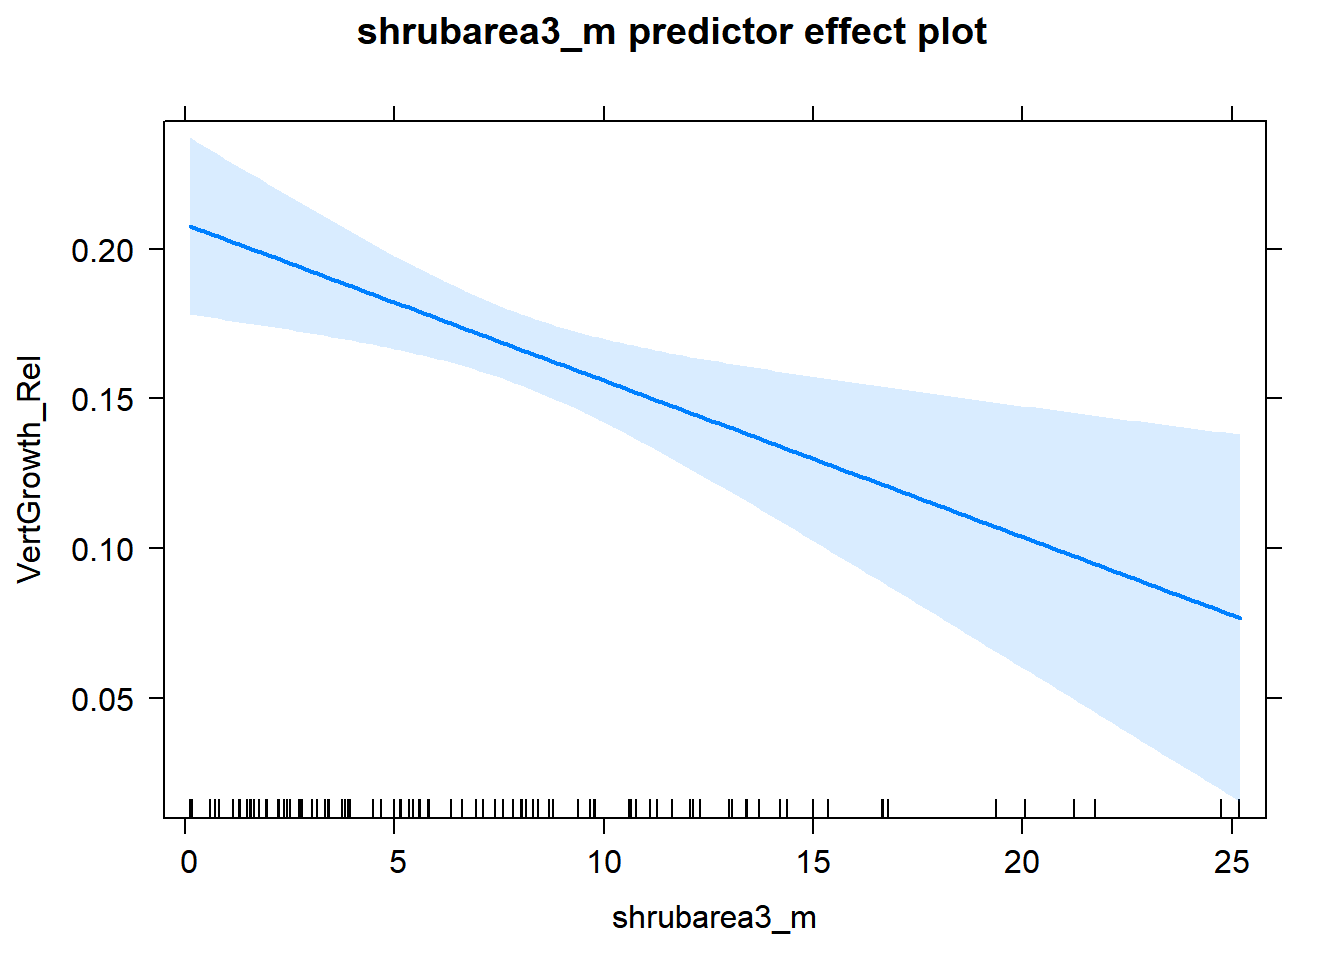
\includegraphics{simulations_files/figure-latex/unnamed-chunk-15-1.pdf}

\section{Simulate across years}\label{simulate-across-years}

\begin{Shaded}
\begin{Highlighting}[]
\NormalTok{time <-}\StringTok{ }\KeywordTok{Sys.time}\NormalTok{()}
\KeywordTok{suppressMessages}\NormalTok{(}\KeywordTok{sim}\NormalTok{(years))}
\KeywordTok{print}\NormalTok{(}\KeywordTok{paste}\NormalTok{(}\StringTok{"One simulation run took"}\NormalTok{, }\KeywordTok{Sys.time}\NormalTok{()}\OperatorTok{-}\NormalTok{time, }\StringTok{"seconds"}\NormalTok{))}
\end{Highlighting}
\end{Shaded}

\begin{verbatim}
## [1] "One simulation run took 5.54435586929321 seconds"
\end{verbatim}

\subsection{Tests}\label{tests}

\subsubsection{Shrub growth patterns}\label{shrub-growth-patterns}

\begin{Shaded}
\begin{Highlighting}[]
\KeywordTok{ggplot}\NormalTok{(dfsimall }\OperatorTok\StringTok{ }\KeywordTok{filter}\NormalTok{(Species }\OperatorTok{==}\StringTok{ "ABCO"}\NormalTok{))}\OperatorTok{+}
\StringTok{  }\KeywordTok{geom_line}\NormalTok{(}\KeywordTok{aes}\NormalTok{(}\DataTypeTok{x =}\NormalTok{ Years, }\DataTypeTok{y =}\NormalTok{ Ht1.}\DecValTok{3}\NormalTok{, }\DataTypeTok{col =}\NormalTok{ ShrubSpp03, }\DataTypeTok{group =}\NormalTok{ Sdlg))}\OperatorTok{+}
\StringTok{  }\KeywordTok{theme_bw}\NormalTok{()}
\end{Highlighting}
\end{Shaded}

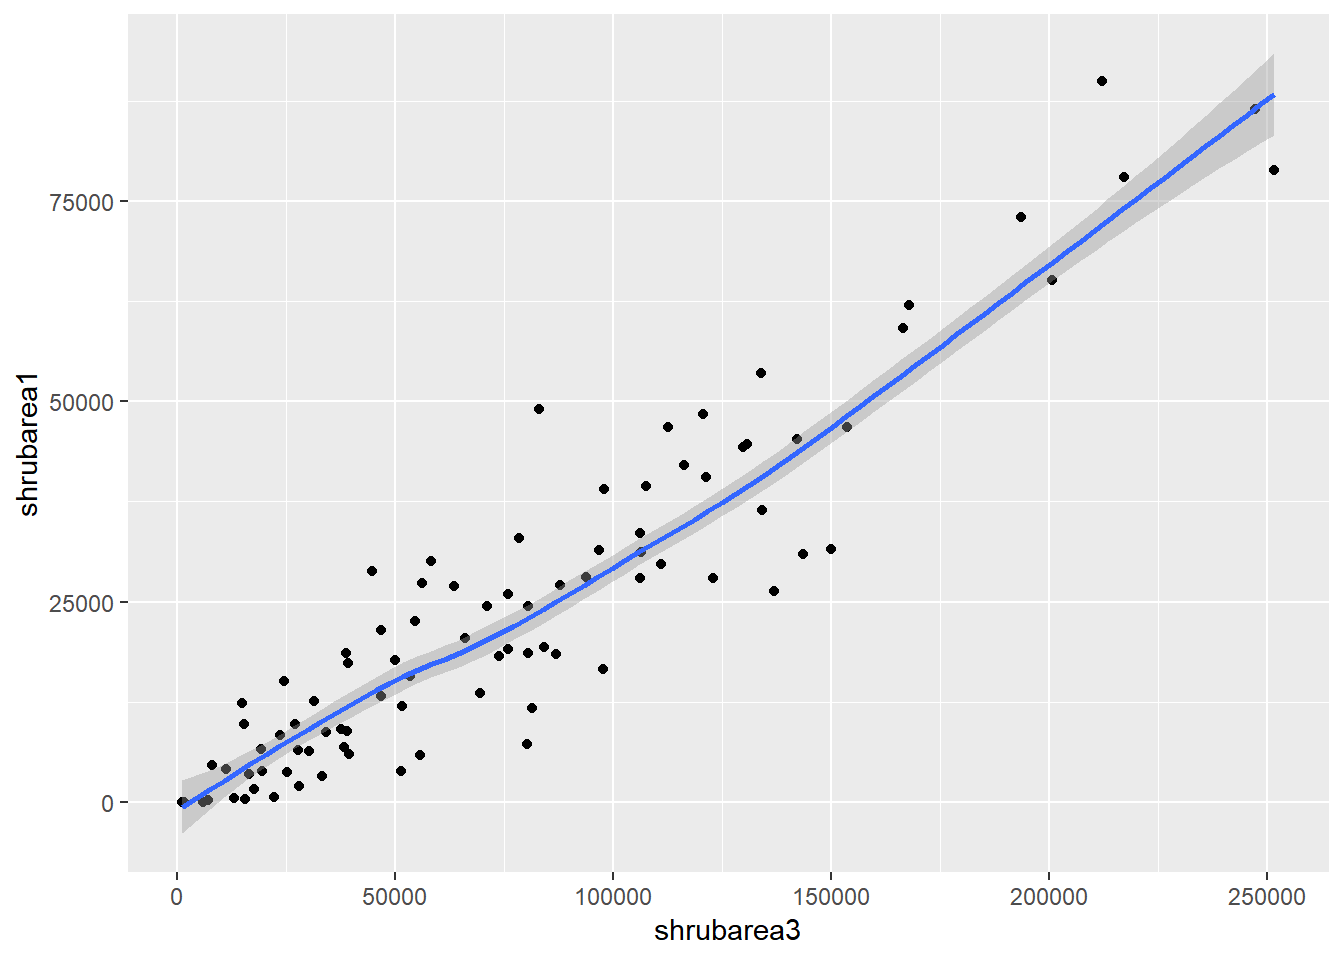
\includegraphics{simulations_files/figure-latex/unnamed-chunk-17-1.pdf}

\begin{Shaded}
\begin{Highlighting}[]
\KeywordTok{ggplot}\NormalTok{(dfsimall }\OperatorTok\StringTok{ }\KeywordTok{filter}\NormalTok{(Species }\OperatorTok{==}\StringTok{ "PIPO"}\NormalTok{))}\OperatorTok{+}
\StringTok{  }\KeywordTok{geom_line}\NormalTok{(}\KeywordTok{aes}\NormalTok{(}\DataTypeTok{x =}\NormalTok{ Years, }\DataTypeTok{y =}\NormalTok{ Ht1.}\DecValTok{3}\NormalTok{, }\DataTypeTok{col =}\NormalTok{ ShrubSpp03, }\DataTypeTok{group =}\NormalTok{ Sdlg))}\OperatorTok{+}
\StringTok{  }\KeywordTok{theme_bw}\NormalTok{()}
\end{Highlighting}
\end{Shaded}

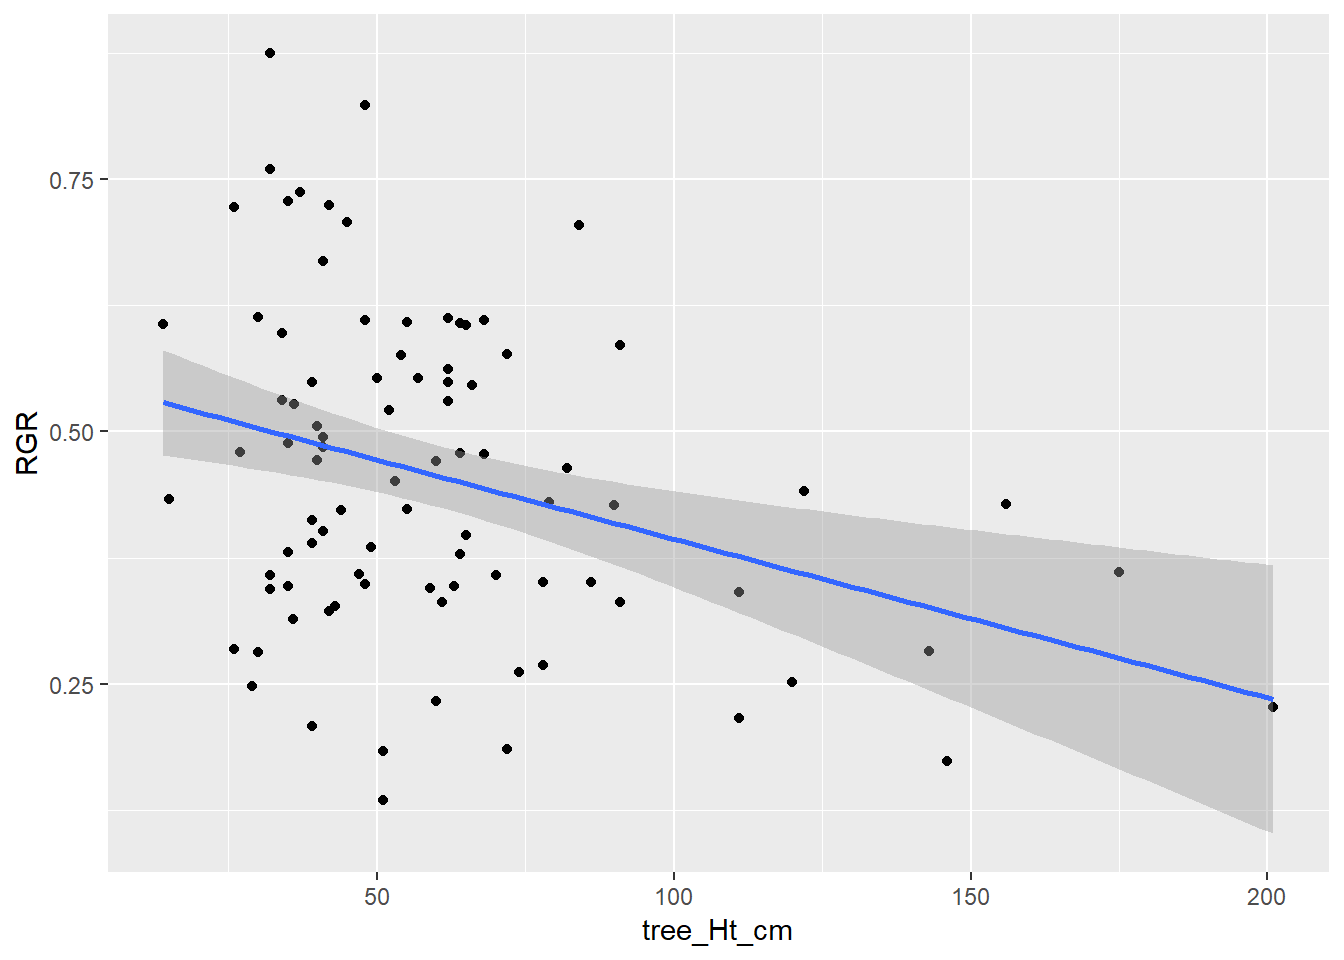
\includegraphics{simulations_files/figure-latex/unnamed-chunk-18-1.pdf}

\subsubsection{Diameter growth patterns}\label{diameter-growth-patterns}

\begin{Shaded}
\begin{Highlighting}[]
\KeywordTok{ggplot}\NormalTok{(dfsimall, }\KeywordTok{aes}\NormalTok{(}\DataTypeTok{x =}\NormalTok{ Years, }\DataTypeTok{y =}\NormalTok{ dia.cm, }\DataTypeTok{col =}\NormalTok{ Species, }\DataTypeTok{group =}\NormalTok{ Sdlg))}\OperatorTok{+}
\StringTok{  }\KeywordTok{geom_line}\NormalTok{(}\DataTypeTok{alpha =}\NormalTok{ .}\DecValTok{3}\NormalTok{)}\OperatorTok{+}
\StringTok{  }\KeywordTok{theme_bw}\NormalTok{()}\OperatorTok{+}
\StringTok{  }\KeywordTok{geom_smooth}\NormalTok{(}\KeywordTok{aes}\NormalTok{(}\DataTypeTok{x =}\NormalTok{ Years, }\DataTypeTok{y =}\NormalTok{ dia.cm, }\DataTypeTok{col =}\NormalTok{ Species, }\DataTypeTok{group =}\NormalTok{ Species))}
\end{Highlighting}
\end{Shaded}

\begin{verbatim}
## `geom_smooth()` using method = 'gam' and formula 'y ~ s(x, bs = "cs")'
\end{verbatim}

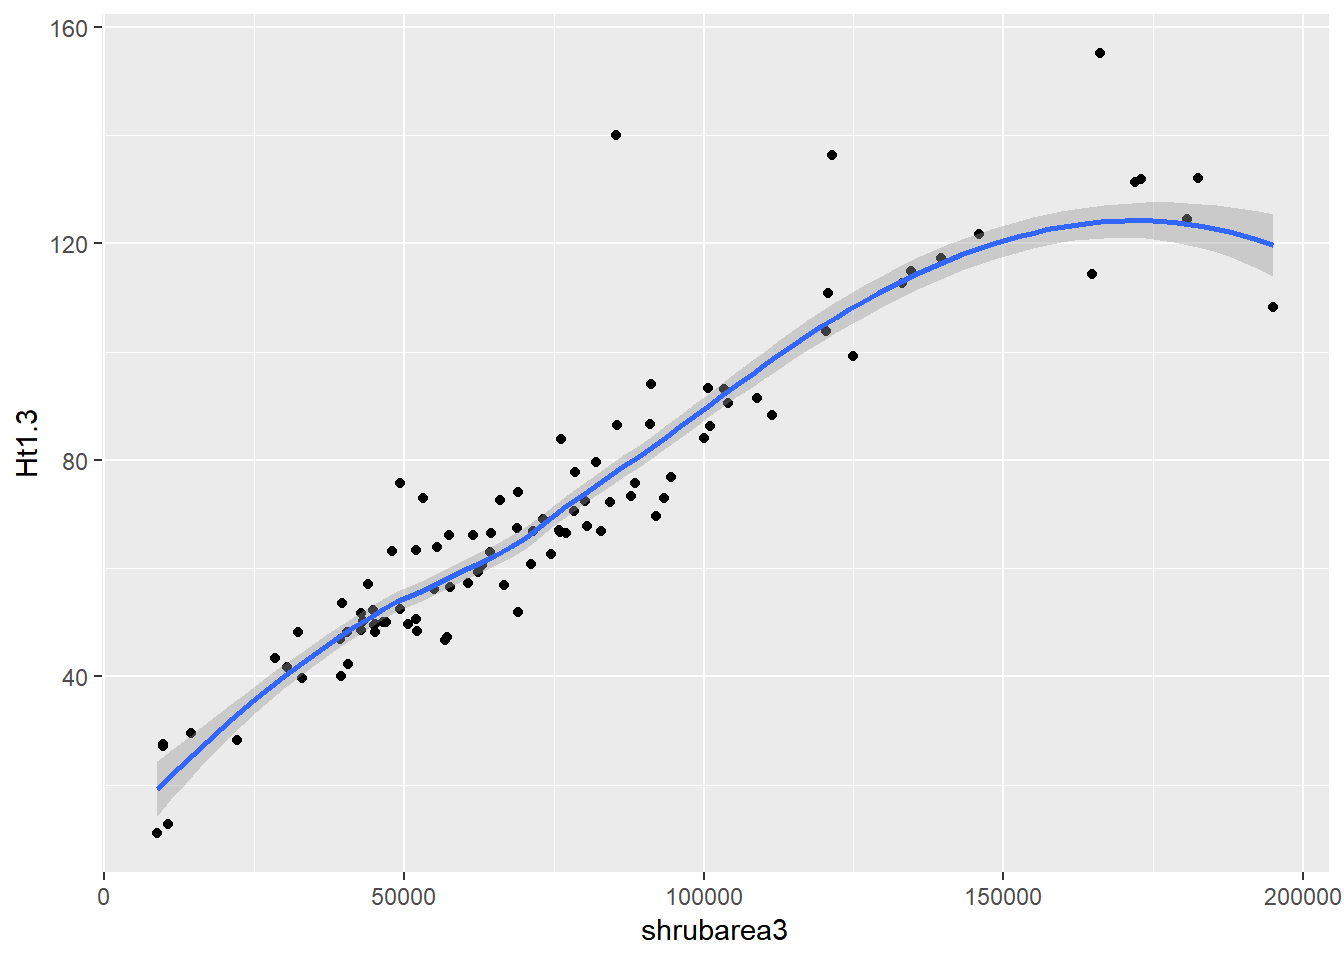
\includegraphics{simulations_files/figure-latex/unnamed-chunk-19-1.pdf}

\subsubsection{Height growth patterns}\label{height-growth-patterns}

\begin{Shaded}
\begin{Highlighting}[]
\KeywordTok{ggplot}\NormalTok{(dfsimall, }\KeywordTok{aes}\NormalTok{(}\DataTypeTok{x =}\NormalTok{ Years, }\DataTypeTok{y =}\NormalTok{ Ht_cm1, }\DataTypeTok{col =}\NormalTok{ Species, }\DataTypeTok{group =}\NormalTok{ Sdlg))}\OperatorTok{+}
\StringTok{  }\KeywordTok{geom_line}\NormalTok{(}\DataTypeTok{alpha =}\NormalTok{ .}\DecValTok{3}\NormalTok{)}\OperatorTok{+}
\StringTok{  }\KeywordTok{theme_bw}\NormalTok{()}\OperatorTok{+}
\StringTok{  }\KeywordTok{geom_smooth}\NormalTok{(}\KeywordTok{aes}\NormalTok{(}\DataTypeTok{x =}\NormalTok{ Years, }\DataTypeTok{y =}\NormalTok{ Ht_cm1, }\DataTypeTok{col =}\NormalTok{ Species, }\DataTypeTok{group =}\NormalTok{ Species))}
\end{Highlighting}
\end{Shaded}

\begin{verbatim}
## `geom_smooth()` using method = 'gam' and formula 'y ~ s(x, bs = "cs")'
\end{verbatim}

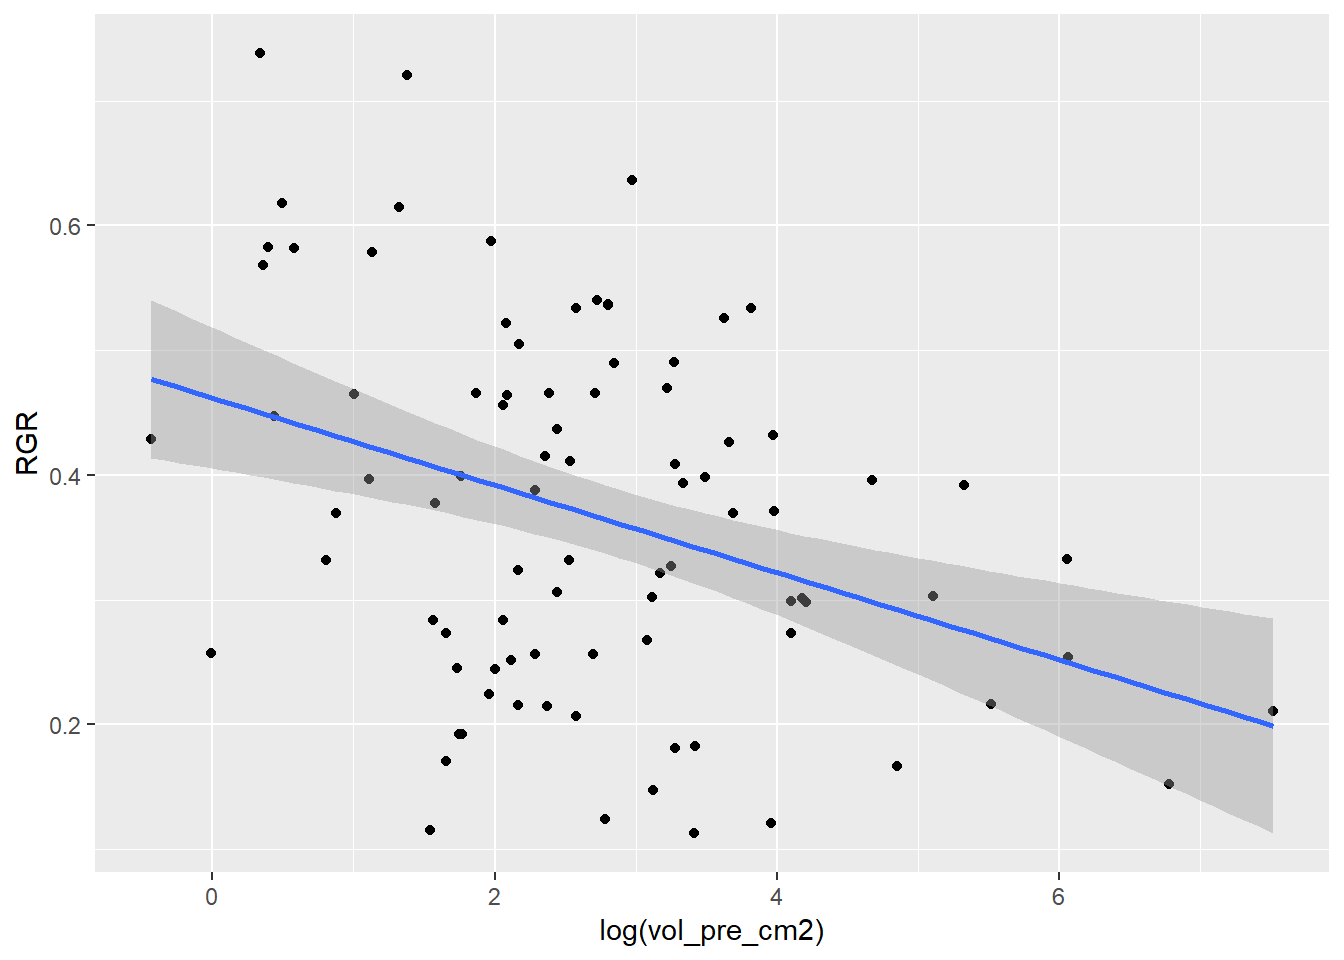
\includegraphics{simulations_files/figure-latex/unnamed-chunk-20-1.pdf}

\subsubsection{Diameter::Height growth
patterns}\label{diameterheight-growth-patterns}

\begin{Shaded}
\begin{Highlighting}[]
\KeywordTok{ggplot}\NormalTok{(dfsimall, }\KeywordTok{aes}\NormalTok{(}\DataTypeTok{x =}\NormalTok{ Years, }\DataTypeTok{y =}\NormalTok{ dia.cm}\OperatorTok{/}\NormalTok{Ht_cm1, }\DataTypeTok{col =}\NormalTok{ Species, }\DataTypeTok{group =}\NormalTok{ Sdlg))}\OperatorTok{+}
\StringTok{  }\KeywordTok{geom_line}\NormalTok{(}\DataTypeTok{alpha =}\NormalTok{ .}\DecValTok{3}\NormalTok{)}\OperatorTok{+}
\StringTok{  }\KeywordTok{theme_bw}\NormalTok{()}\OperatorTok{+}
\StringTok{  }\KeywordTok{geom_smooth}\NormalTok{(}\KeywordTok{aes}\NormalTok{(}\DataTypeTok{x =}\NormalTok{ Years, }\DataTypeTok{y =}\NormalTok{ dia.cm}\OperatorTok{/}\NormalTok{Ht_cm1, }\DataTypeTok{col =}\NormalTok{ Species, }\DataTypeTok{group =}\NormalTok{ Species))}
\end{Highlighting}
\end{Shaded}

\begin{verbatim}
## `geom_smooth()` using method = 'gam' and formula 'y ~ s(x, bs = "cs")'
\end{verbatim}

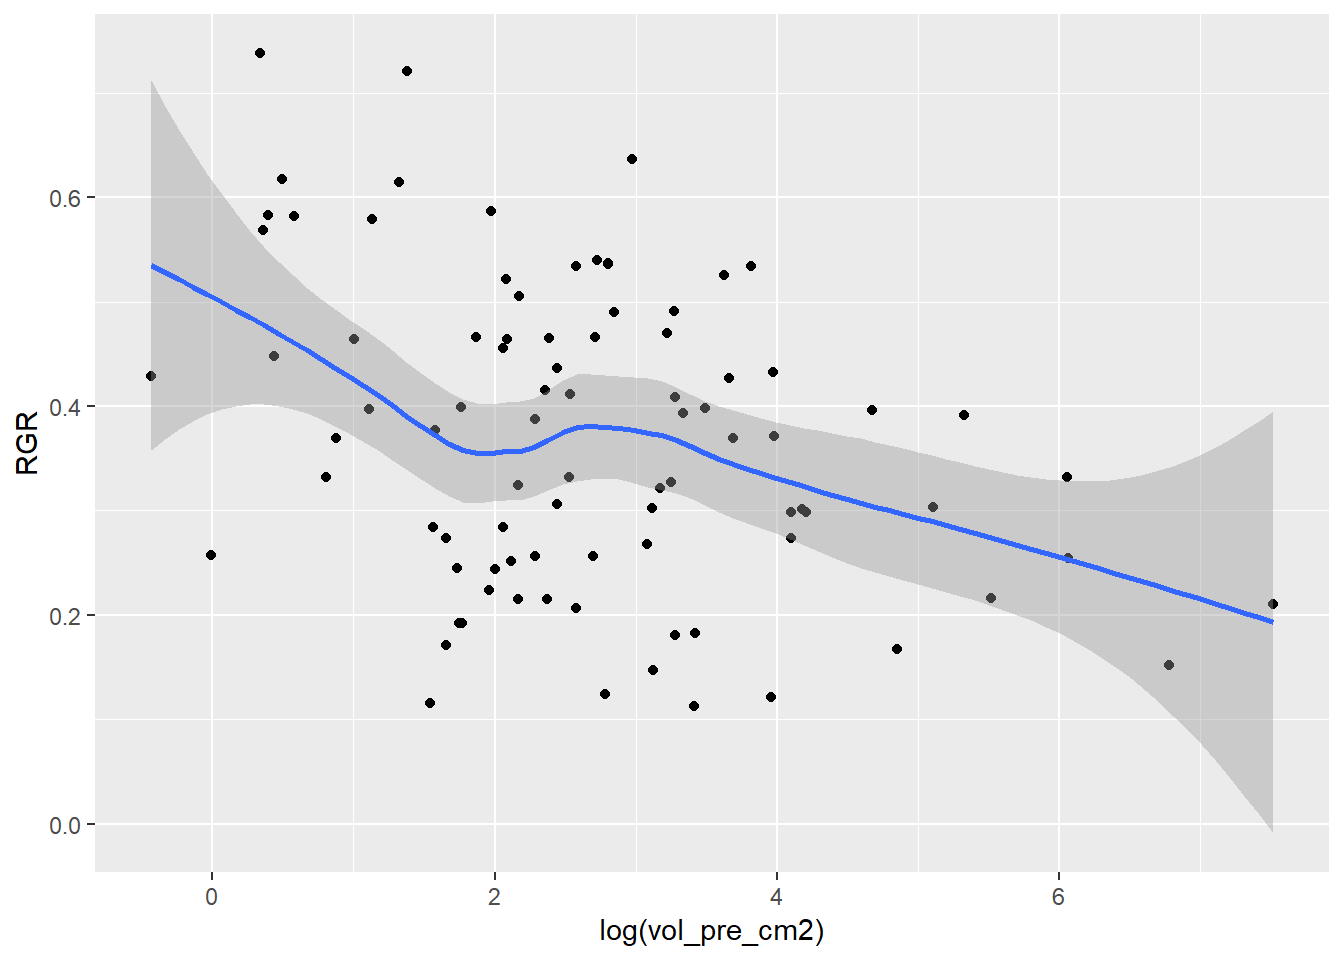
\includegraphics{simulations_files/figure-latex/unnamed-chunk-21-1.pdf}

\subsubsection{Diameter:height}\label{diameterheight}

\begin{Shaded}
\begin{Highlighting}[]
\KeywordTok{ggplot}\NormalTok{(dfsimall }\OperatorTok\StringTok{ }\KeywordTok{filter}\NormalTok{(Years}\OperatorTok{==}\DecValTok{10}\NormalTok{))}\OperatorTok{+}
\StringTok{  }\KeywordTok{geom_histogram}\NormalTok{(}\KeywordTok{aes}\NormalTok{(dia.cm}\OperatorTok{/}\NormalTok{Ht_cm1, }\DataTypeTok{bins =} \DecValTok{20}\NormalTok{))}
\end{Highlighting}
\end{Shaded}

\begin{verbatim}
## Warning: Ignoring unknown aesthetics: bins
\end{verbatim}

\begin{verbatim}
## `stat_bin()` using `bins = 30`. Pick better value with `binwidth`.
\end{verbatim}

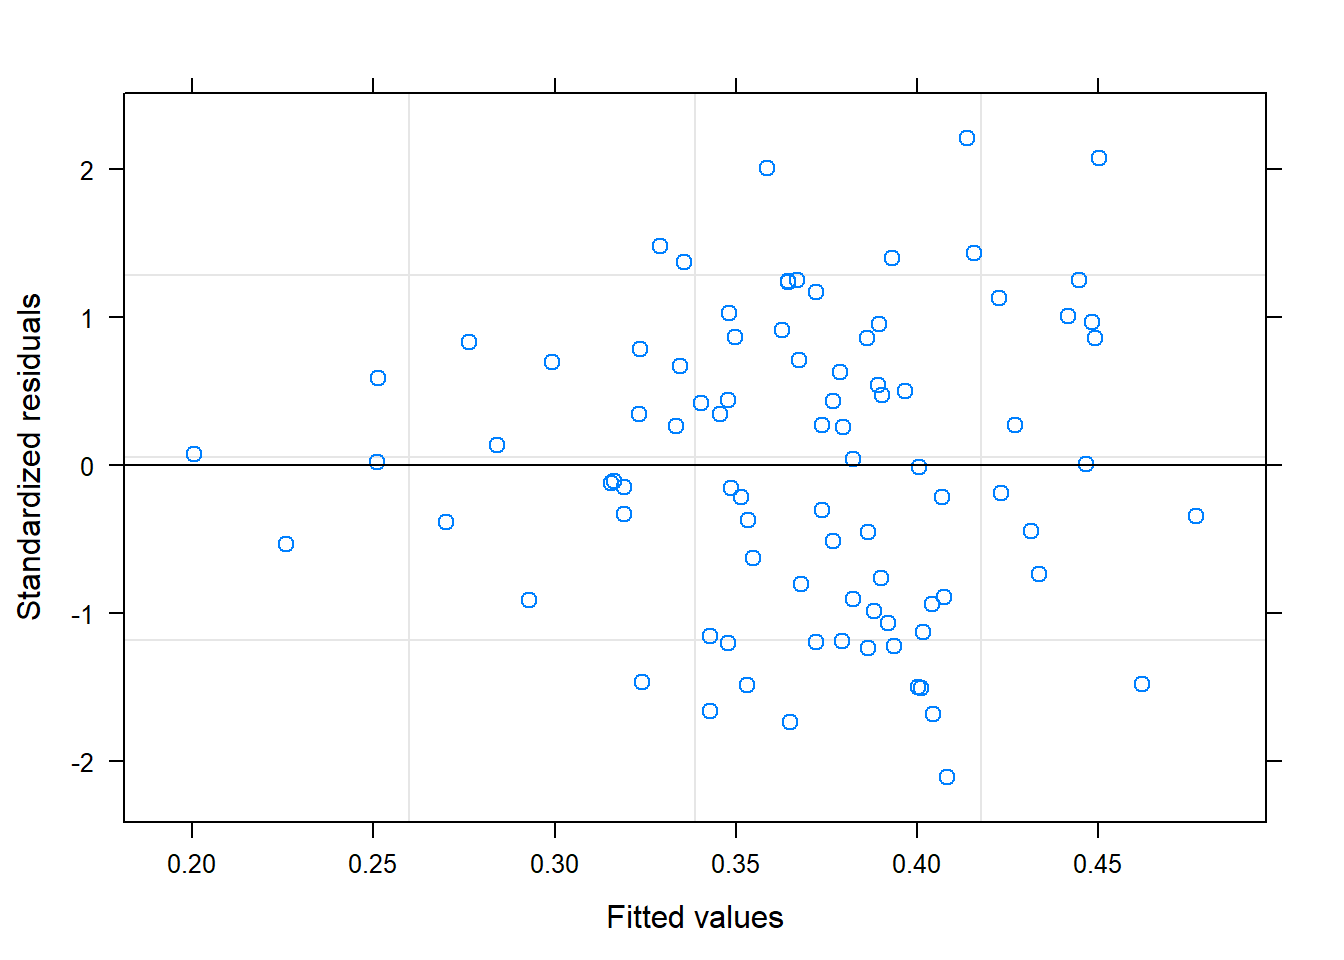
\includegraphics{simulations_files/figure-latex/unnamed-chunk-22-1.pdf}

\begin{Shaded}
\begin{Highlighting}[]
\KeywordTok{ggplot}\NormalTok{(dfsimall }\OperatorTok\StringTok{ }\KeywordTok{filter}\NormalTok{(Years}\OperatorTok{==}\DecValTok{20}\NormalTok{))}\OperatorTok{+}
\StringTok{  }\KeywordTok{geom_histogram}\NormalTok{(}\KeywordTok{aes}\NormalTok{(dia.cm}\OperatorTok{/}\NormalTok{Ht_cm1, }\DataTypeTok{bins =} \DecValTok{20}\NormalTok{))}
\end{Highlighting}
\end{Shaded}

\begin{verbatim}
## Warning: Ignoring unknown aesthetics: bins
\end{verbatim}

\begin{verbatim}
## `stat_bin()` using `bins = 30`. Pick better value with `binwidth`.
\end{verbatim}

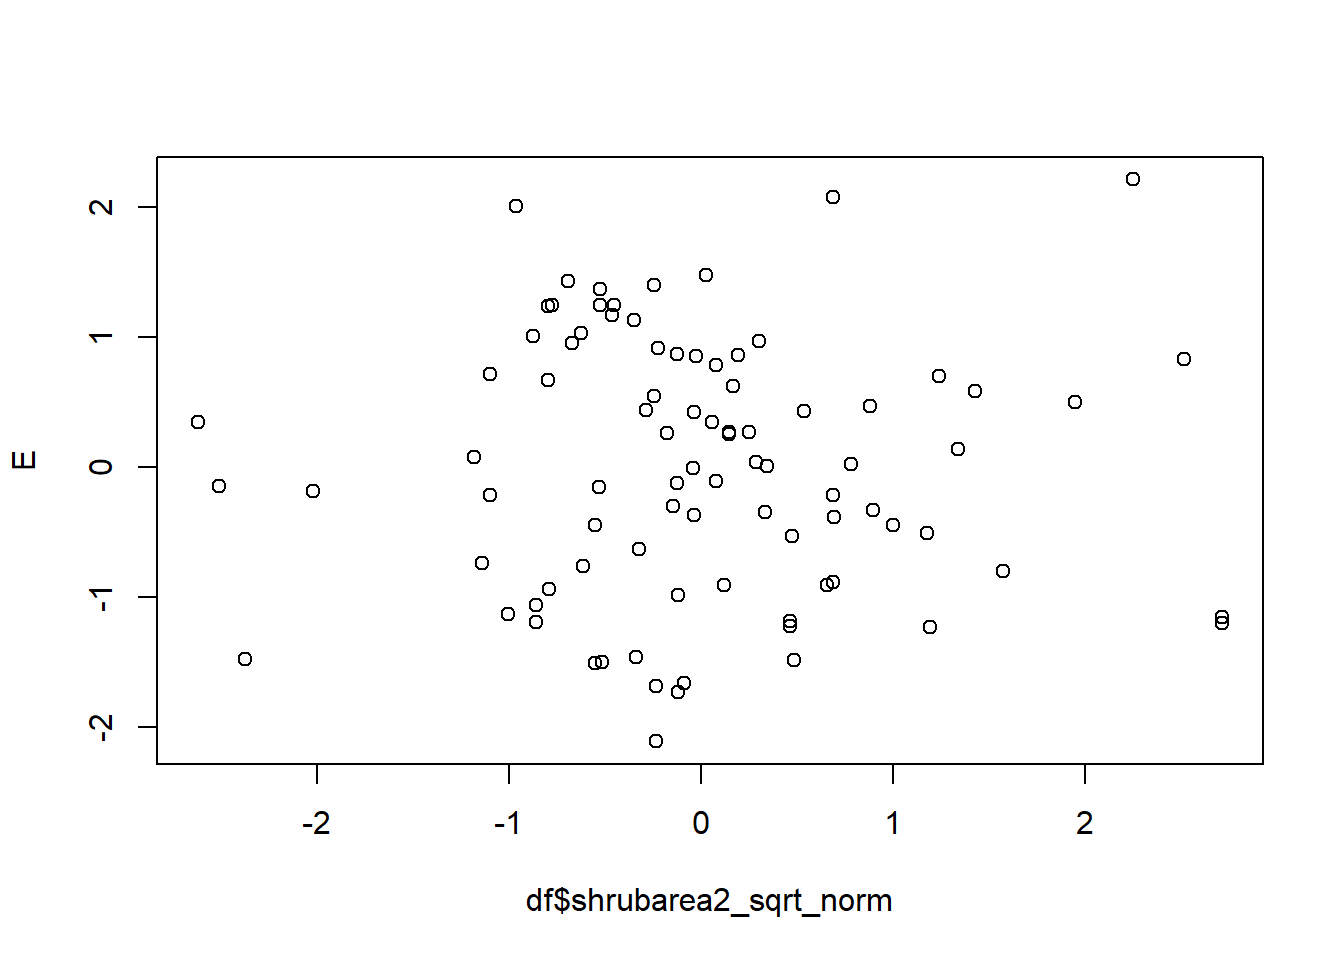
\includegraphics{simulations_files/figure-latex/unnamed-chunk-22-2.pdf}

\subsubsection{Diameter and height
boxplots}\label{diameter-and-height-boxplots}

\begin{Shaded}
\begin{Highlighting}[]
\KeywordTok{ggplot}\NormalTok{(dfsimall)}\OperatorTok{+}
\StringTok{  }\KeywordTok{geom_boxplot}\NormalTok{(}\KeywordTok{aes}\NormalTok{(}\DataTypeTok{x =} \KeywordTok{as.factor}\NormalTok{(Years), }\DataTypeTok{y =}\NormalTok{ dia.cm, }\DataTypeTok{fill =}\NormalTok{ Species))}\OperatorTok{+}
\StringTok{  }\KeywordTok{theme_minimal}\NormalTok{()}\OperatorTok{+}
\StringTok{  }\KeywordTok{xlab}\NormalTok{(}\StringTok{"Years"}\NormalTok{)}\OperatorTok{+}
\StringTok{  }\KeywordTok{ylab}\NormalTok{(}\StringTok{"Diameter (cm)"}\NormalTok{)}\OperatorTok{+}
\StringTok{  }\KeywordTok{theme}\NormalTok{(}\DataTypeTok{text =} \KeywordTok{element_text}\NormalTok{(}\DataTypeTok{size =} \DecValTok{20}\NormalTok{))}
\end{Highlighting}
\end{Shaded}

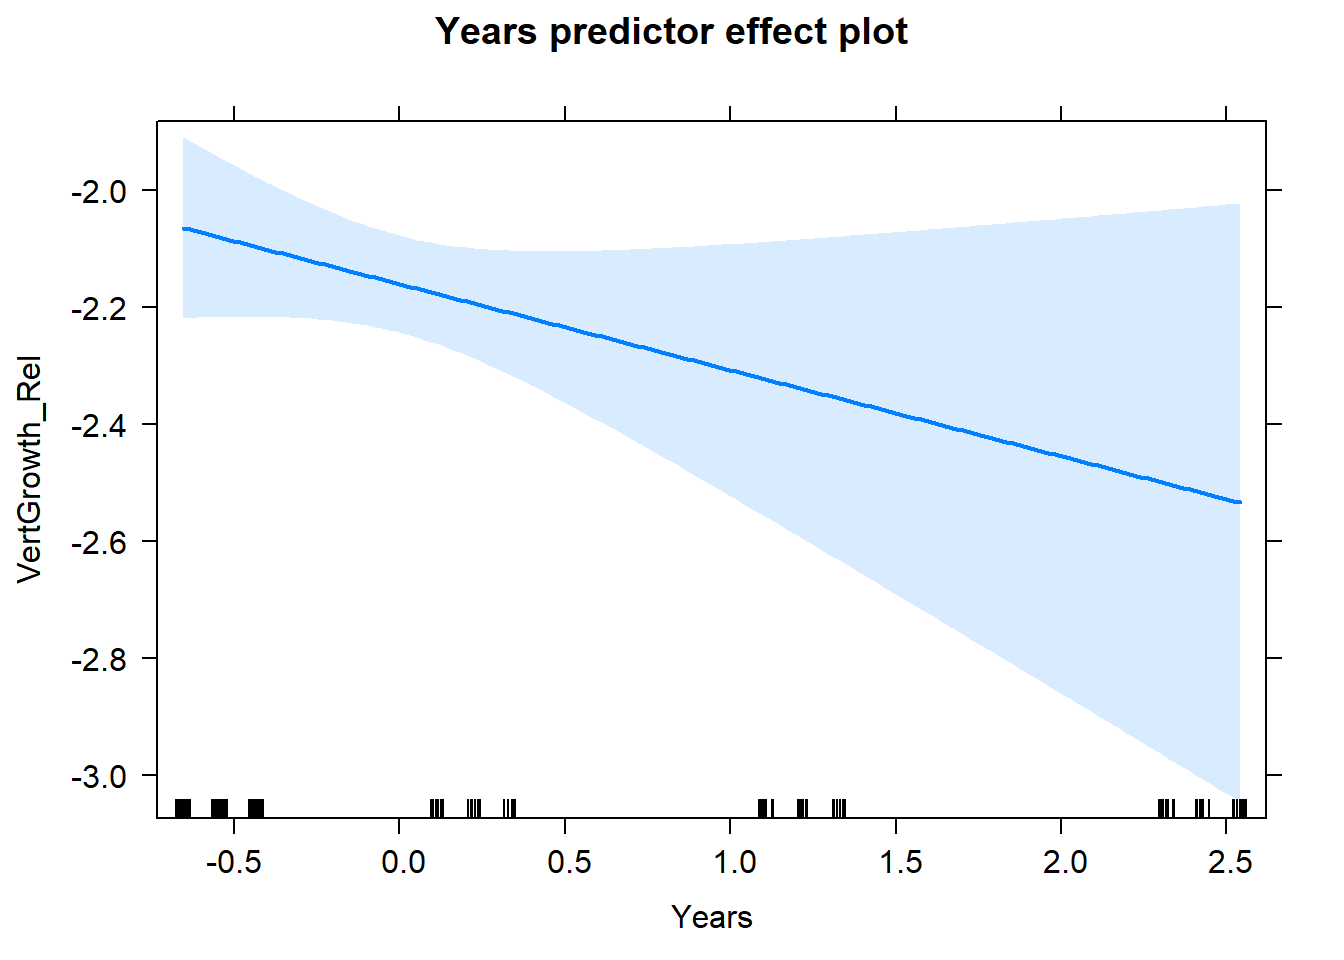
\includegraphics{simulations_files/figure-latex/unnamed-chunk-23-1.pdf}

\begin{Shaded}
\begin{Highlighting}[]
\KeywordTok{ggplot}\NormalTok{(dfsimall)}\OperatorTok{+}
\StringTok{  }\KeywordTok{geom_boxplot}\NormalTok{(}\KeywordTok{aes}\NormalTok{(}\DataTypeTok{x =} \KeywordTok{as.factor}\NormalTok{(Years), }\DataTypeTok{y =}\NormalTok{ Ht_cm1, }\DataTypeTok{fill =}\NormalTok{ Species))}\OperatorTok{+}
\StringTok{  }\KeywordTok{theme_minimal}\NormalTok{()}\OperatorTok{+}
\StringTok{  }\KeywordTok{xlab}\NormalTok{(}\StringTok{"Years"}\NormalTok{)}\OperatorTok{+}
\StringTok{  }\KeywordTok{ylab}\NormalTok{(}\StringTok{"Height (cm)"}\NormalTok{)}\OperatorTok{+}
\StringTok{  }\KeywordTok{theme}\NormalTok{(}\DataTypeTok{text =} \KeywordTok{element_text}\NormalTok{(}\DataTypeTok{size =} \DecValTok{20}\NormalTok{))}
\end{Highlighting}
\end{Shaded}

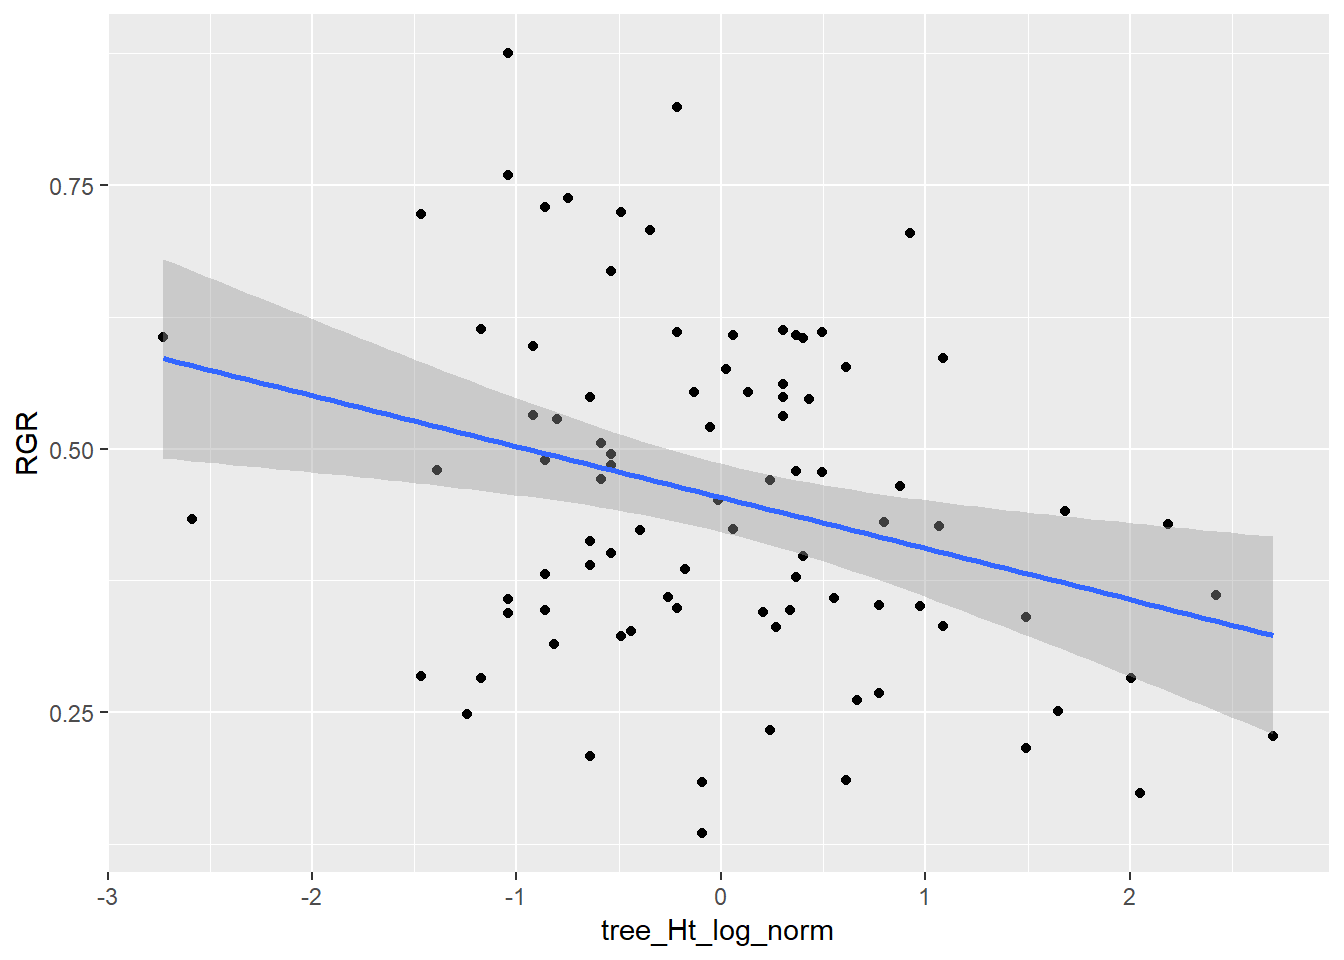
\includegraphics{simulations_files/figure-latex/unnamed-chunk-24-1.pdf}

\subsection{Plot shrub patch
spatially}\label{plot-shrub-patch-spatially}

\begin{Shaded}
\begin{Highlighting}[]
\NormalTok{pts.sf.pipo.graph <-}\StringTok{ }\NormalTok{pts.sf.pipo }\OperatorTok\StringTok{ }
\StringTok{  }\KeywordTok{rename}\NormalTok{(}\StringTok{"Pine height (cm)"}\NormalTok{ =}\StringTok{ }\NormalTok{Ht_cm1)}
\NormalTok{pts.sf.abco.graph <-}\StringTok{ }\NormalTok{pts.sf.abco }\OperatorTok\StringTok{ }
\StringTok{  }\KeywordTok{rename}\NormalTok{(}\StringTok{"Fir height (cm)"}\NormalTok{ =}\StringTok{ }\NormalTok{Ht_cm1)}
\end{Highlighting}
\end{Shaded}

\begin{Shaded}
\begin{Highlighting}[]
\KeywordTok{tm_shape}\NormalTok{(p)}\OperatorTok{+}
\StringTok{  }\KeywordTok{tm_borders}\NormalTok{(}\DataTypeTok{col =} \StringTok{"black"}\NormalTok{, }\DataTypeTok{lwd=} \DecValTok{5}\NormalTok{)}\OperatorTok{+}
\KeywordTok{tm_shape}\NormalTok{(r)}\OperatorTok{+}
\StringTok{  }\KeywordTok{tm_raster}\NormalTok{(}\DataTypeTok{col =} \StringTok{"sqrt_shrubarea3"}\NormalTok{, }\DataTypeTok{title =} \StringTok{"Shrub competition index"}\NormalTok{, }\DataTypeTok{palette =} \StringTok{"Greys"}\NormalTok{, }\DataTypeTok{alpha =}\NormalTok{ .}\DecValTok{5}\NormalTok{)}\OperatorTok{+}
\KeywordTok{tm_shape}\NormalTok{(r)}\OperatorTok{+}
\StringTok{  }\KeywordTok{tm_raster}\NormalTok{(}\DataTypeTok{col =} \StringTok{"ShrubSpp03"}\NormalTok{, }\DataTypeTok{alpha =}\NormalTok{ .}\DecValTok{7}\NormalTok{, }\DataTypeTok{title =} \StringTok{"Shrub species"}\NormalTok{, }\DataTypeTok{palette =} \StringTok{"Pastel1"}\NormalTok{)}\OperatorTok{+}
\StringTok{  }\KeywordTok{tm_layout}\NormalTok{(}\DataTypeTok{asp=}\DecValTok{1}\OperatorTok{:}\DecValTok{1}\NormalTok{, }\DataTypeTok{legend.outside =}\NormalTok{ T, }\DataTypeTok{legend.title.size =} \DecValTok{4}\NormalTok{, }\DataTypeTok{legend.text.size =} \DecValTok{2}\NormalTok{)}\OperatorTok{+}
\KeywordTok{tm_shape}\NormalTok{(pts.sf.pipo.graph)}\OperatorTok{+}
\StringTok{  }\KeywordTok{tm_symbols}\NormalTok{(}\DataTypeTok{size =} \StringTok{"Pine height (cm)"}\NormalTok{, }\DataTypeTok{col =} \StringTok{"#DCC960"}\NormalTok{, }\DataTypeTok{size.max =} \DecValTok{300}\NormalTok{, }\DataTypeTok{border.lwd =} \DecValTok{3}\NormalTok{)}\OperatorTok{+}
\KeywordTok{tm_shape}\NormalTok{(pts.sf.abco.graph)}\OperatorTok{+}
\StringTok{  }\KeywordTok{tm_symbols}\NormalTok{(}\DataTypeTok{size =} \StringTok{"Fir height (cm)"}\NormalTok{, }\DataTypeTok{col =} \StringTok{"#899DA4"}\NormalTok{, }\DataTypeTok{size.max =} \DecValTok{300}\NormalTok{, }\DataTypeTok{border.lwd =} \DecValTok{3}\NormalTok{)}
\end{Highlighting}
\end{Shaded}

\begin{verbatim}
## Note that 6 values of the variable "Pine height (cm)" (the highest being 477.914588296625) are larger than size.max, which is currently set to 300. It is recommended to set size.max to at least 477.914588296625. Another option is to set size.lim = c(0, 300), which truncates the size of the 6 larger symbols. Use the scale argument to increase the size of all symbols.
\end{verbatim}

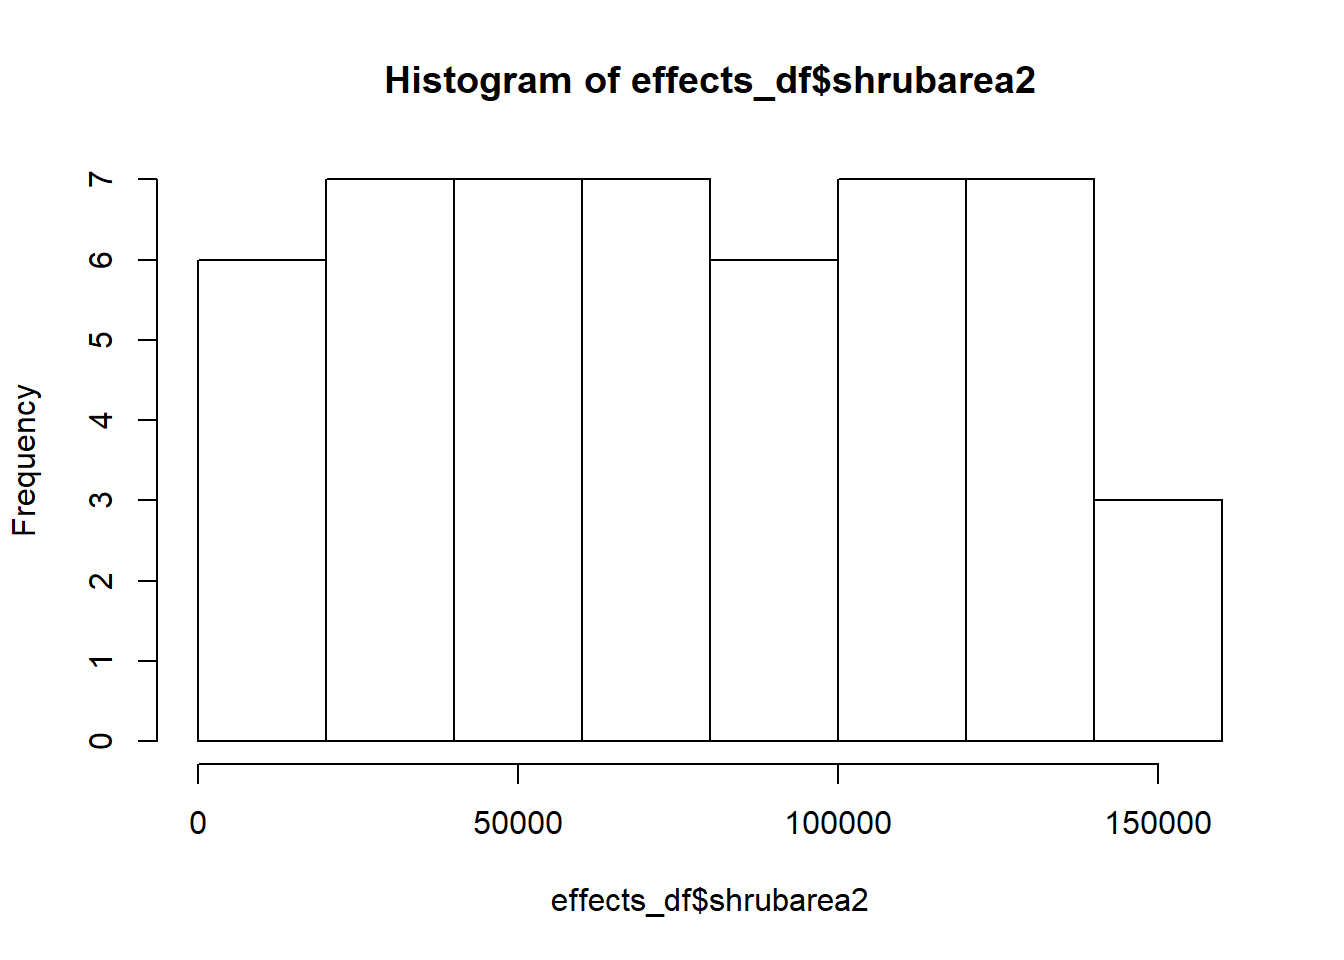
\includegraphics{simulations_files/figure-latex/unnamed-chunk-26-1.pdf}

\section{Iterate}\label{iterate}

\begin{Shaded}
\begin{Highlighting}[]
\NormalTok{time <-}\StringTok{ }\KeywordTok{Sys.time}\NormalTok{()}
\KeywordTok{iterate}\NormalTok{(iterations)}
\end{Highlighting}
\end{Shaded}

\begin{verbatim}
## [1] "Done with 10 iterations in 1 minutes"
## [1] "Done with 20 iterations in 1.9 minutes"
## [1] "Done with 30 iterations in 2.8 minutes"
## [1] "Done with 40 iterations in 3.6 minutes"
## [1] "Done with 50 iterations in 4.5 minutes"
## [1] "Done with 60 iterations in 5.4 minutes"
## [1] "Done with 70 iterations in 6.2 minutes"
## [1] "Done with 80 iterations in 7.1 minutes"
## [1] "Done with 90 iterations in 8 minutes"
## [1] "Done with 100 iterations in 8.8 minutes"
## [1] "Done with 110 iterations in 9.7 minutes"
## [1] "Done with 120 iterations in 10.6 minutes"
## [1] "Done with 130 iterations in 11.5 minutes"
## [1] "Done with 140 iterations in 12.4 minutes"
## [1] "Done with 150 iterations in 13.3 minutes"
## [1] "Done with 160 iterations in 14.1 minutes"
## [1] "Done with 170 iterations in 15 minutes"
## [1] "Done with 180 iterations in 15.9 minutes"
## [1] "Done with 190 iterations in 16.8 minutes"
## [1] "Done with 200 iterations in 17.7 minutes"
## [1] "Done with 210 iterations in 18.5 minutes"
## [1] "Done with 220 iterations in 19.4 minutes"
## [1] "Done with 230 iterations in 20.3 minutes"
## [1] "Done with 240 iterations in 21.2 minutes"
## [1] "Done with 250 iterations in 22.1 minutes"
## [1] "Done with 260 iterations in 23 minutes"
## [1] "Done with 270 iterations in 23.8 minutes"
## [1] "Done with 280 iterations in 24.7 minutes"
## [1] "Done with 290 iterations in 25.6 minutes"
## [1] "Done with 300 iterations in 26.5 minutes"
## [1] "Done with 310 iterations in 27.4 minutes"
## [1] "Done with 320 iterations in 28.3 minutes"
## [1] "Done with 330 iterations in 29.2 minutes"
## [1] "Done with 340 iterations in 30.1 minutes"
## [1] "Done with 350 iterations in 31 minutes"
## [1] "Done with 360 iterations in 31.9 minutes"
## [1] "Done with 370 iterations in 32.8 minutes"
## [1] "Done with 380 iterations in 33.7 minutes"
## [1] "Done with 390 iterations in 34.6 minutes"
## [1] "Done with 400 iterations in 35.5 minutes"
## [1] "Done with 410 iterations in 36.4 minutes"
## [1] "Done with 420 iterations in 37.3 minutes"
## [1] "Done with 430 iterations in 38.2 minutes"
## [1] "Done with 440 iterations in 39.1 minutes"
## [1] "Done with 450 iterations in 40 minutes"
## [1] "Done with 460 iterations in 40.9 minutes"
## [1] "Done with 470 iterations in 41.8 minutes"
## [1] "Done with 480 iterations in 42.7 minutes"
## [1] "Done with 490 iterations in 43.6 minutes"
## [1] "Done with 500 iterations in 44.5 minutes"
## [1] "Done with 510 iterations in 45.5 minutes"
## [1] "Done with 520 iterations in 46.4 minutes"
## [1] "Done with 530 iterations in 47.3 minutes"
## [1] "Done with 540 iterations in 48.2 minutes"
## [1] "Done with 550 iterations in 49.1 minutes"
## [1] "Done with 560 iterations in 50.1 minutes"
## [1] "Done with 570 iterations in 51 minutes"
## [1] "Done with 580 iterations in 52 minutes"
## [1] "Done with 590 iterations in 52.9 minutes"
## [1] "Done with 600 iterations in 53.8 minutes"
## [1] "Done with 610 iterations in 54.8 minutes"
## [1] "Done with 620 iterations in 55.7 minutes"
## [1] "Done with 630 iterations in 56.7 minutes"
## [1] "Done with 640 iterations in 57.6 minutes"
## [1] "Done with 650 iterations in 58.5 minutes"
## [1] "Done with 660 iterations in 59.5 minutes"
## [1] "Done with 670 iterations in 1 minutes"
## [1] "Done with 680 iterations in 1 minutes"
## [1] "Done with 690 iterations in 1 minutes"
## [1] "Done with 700 iterations in 1.1 minutes"
## [1] "Done with 710 iterations in 1.1 minutes"
## [1] "Done with 720 iterations in 1.1 minutes"
## [1] "Done with 730 iterations in 1.1 minutes"
## [1] "Done with 740 iterations in 1.1 minutes"
## [1] "Done with 750 iterations in 1.1 minutes"
## [1] "Done with 760 iterations in 1.2 minutes"
## [1] "Done with 770 iterations in 1.2 minutes"
## [1] "Done with 780 iterations in 1.2 minutes"
## [1] "Done with 790 iterations in 1.2 minutes"
## [1] "Done with 800 iterations in 1.2 minutes"
## [1] "Done with 810 iterations in 1.2 minutes"
## [1] "Done with 820 iterations in 1.3 minutes"
## [1] "Done with 830 iterations in 1.3 minutes"
## [1] "Done with 840 iterations in 1.3 minutes"
## [1] "Done with 850 iterations in 1.3 minutes"
## [1] "Done with 860 iterations in 1.3 minutes"
## [1] "Done with 870 iterations in 1.3 minutes"
## [1] "Done with 880 iterations in 1.3 minutes"
## [1] "Done with 890 iterations in 1.4 minutes"
## [1] "Done with 900 iterations in 1.4 minutes"
## [1] "Done with 910 iterations in 1.4 minutes"
## [1] "Done with 920 iterations in 1.4 minutes"
## [1] "Done with 930 iterations in 1.4 minutes"
## [1] "Done with 940 iterations in 1.4 minutes"
## [1] "Done with 950 iterations in 1.5 minutes"
## [1] "Done with 960 iterations in 1.5 minutes"
## [1] "Done with 970 iterations in 1.5 minutes"
## [1] "Done with 980 iterations in 1.5 minutes"
## [1] "Done with 990 iterations in 1.5 minutes"
## [1] "Done with 1000 iterations in 1.5 minutes"
\end{verbatim}

\begin{Shaded}
\begin{Highlighting}[]
\KeywordTok{print}\NormalTok{(}\KeywordTok{paste}\NormalTok{(}\StringTok{"That took"}\NormalTok{, }\KeywordTok{round}\NormalTok{(}\KeywordTok{Sys.time}\NormalTok{()}\OperatorTok{-}\NormalTok{time, }\DecValTok{1}\NormalTok{), }\StringTok{"minutes"}\NormalTok{))}
\end{Highlighting}
\end{Shaded}

\begin{verbatim}
## [1] "That took 1.5 minutes"
\end{verbatim}

\begin{Shaded}
\begin{Highlighting}[]
\NormalTok{dfsimallreps }\OperatorTok\StringTok{ }
\StringTok{  }\KeywordTok{group_by}\NormalTok{(rep) }\OperatorTok\StringTok{ }
\StringTok{  }\KeywordTok{summarize}\NormalTok{(}\KeywordTok{mean}\NormalTok{(Ht_cm1))}
\end{Highlighting}
\end{Shaded}

\begin{verbatim}
## # A tibble: 1,000 x 2
##      rep `mean(Ht_cm1)`
##    <int>          <dbl>
##  1     1           115.
##  2     2           121.
##  3     3           112.
##  4     4           119.
##  5     5           120.
##  6     6           126.
##  7     7           118.
##  8     8           117.
##  9     9           126.
## 10    10           125.
## # ... with 990 more rows
\end{verbatim}

\section{Summarize}\label{summarize}

\subsection{Height by year}\label{height-by-year}

\begin{Shaded}
\begin{Highlighting}[]
\NormalTok{dfsimallreps_summary <-}\StringTok{ }\NormalTok{dfsimallreps }\OperatorTok\StringTok{ }
\StringTok{  }\KeywordTok{ungroup}\NormalTok{() }\OperatorTok
\StringTok{  }\KeywordTok{mutate}\NormalTok{(}\DataTypeTok{rep =} \KeywordTok{as.factor}\NormalTok{(}\KeywordTok{paste}\NormalTok{(rep))) }\OperatorTok\StringTok{ }
\StringTok{  }\KeywordTok{group_by}\NormalTok{(rep, Years, Species) }\OperatorTok\StringTok{ }
\StringTok{  }\KeywordTok{mutate}\NormalTok{(}\DataTypeTok{mean_ht_years =} \KeywordTok{mean}\NormalTok{(Ht_cm1))}
\NormalTok{dfsimallreps_summary }\OperatorTok\StringTok{ }\NormalTok{dplyr}\OperatorTok{::}\KeywordTok{select}\NormalTok{(rep, Years, mean_ht_years) }\OperatorTok\StringTok{ }\KeywordTok{summary}\NormalTok{()}
\end{Highlighting}
\end{Shaded}

\begin{verbatim}
## Adding missing grouping variables: `Species`
\end{verbatim}

\begin{verbatim}
##  Species             rep              Years       mean_ht_years   
##  ABCO:1796350   795    :   3024   Min.   : 9.00   Min.   : 37.16  
##  PIPO:1016822   135    :   3023   1st Qu.:12.00   1st Qu.: 70.59  
##                 979    :   3020   Median :16.00   Median :109.12  
##                 755    :   3013   Mean   :16.78   Mean   :117.64  
##                 408    :   3011   3rd Qu.:21.00   3rd Qu.:156.04  
##                 376    :   3009   Max.   :28.00   Max.   :339.56  
##                 (Other):2795072
\end{verbatim}

\begin{Shaded}
\begin{Highlighting}[]
\KeywordTok{ggplot}\NormalTok{(dfsimallreps_summary, }\KeywordTok{aes}\NormalTok{(}\DataTypeTok{x =} \KeywordTok{as.factor}\NormalTok{(Years), }\DataTypeTok{y =}\NormalTok{ mean_ht_years, }\DataTypeTok{fill =}\NormalTok{ Species, }\DataTypeTok{col =}\NormalTok{ Species))}\OperatorTok{+}
\StringTok{  }\KeywordTok{geom_boxplot}\NormalTok{(}\DataTypeTok{alpha =}\NormalTok{ .}\DecValTok{2}\NormalTok{, }\DataTypeTok{outlier.alpha =}\NormalTok{ .}\DecValTok{02}\NormalTok{)}\OperatorTok{+}
\StringTok{  }\KeywordTok{geom_smooth}\NormalTok{(}\KeywordTok{aes}\NormalTok{(}\DataTypeTok{x =} \KeywordTok{as.factor}\NormalTok{(Years), }\DataTypeTok{y =}\NormalTok{ mean_ht_years, }\DataTypeTok{group =}\NormalTok{ Species, }\DataTypeTok{col =}\NormalTok{ Species), }\DataTypeTok{size =} \DecValTok{1}\NormalTok{)}\OperatorTok{+}
\StringTok{  }\KeywordTok{ggtitle}\NormalTok{(}\StringTok{"Results for 1000 simulations"}\NormalTok{)}\OperatorTok{+}
\StringTok{  }\KeywordTok{xlab}\NormalTok{(}\StringTok{"Years since fire"}\NormalTok{)}\OperatorTok{+}
\StringTok{  }\KeywordTok{ylab}\NormalTok{(}\StringTok{"Average tree ht (cm) by simulation"}\NormalTok{)}\OperatorTok{+}
\StringTok{  }\KeywordTok{theme_bw}\NormalTok{()}\OperatorTok{+}
\StringTok{  }\KeywordTok{scale_color_manual}\NormalTok{(}\DataTypeTok{values =} \KeywordTok{c}\NormalTok{(}\StringTok{"#899DA4"}\NormalTok{, }\StringTok{"#9A8822"}\NormalTok{), }\DataTypeTok{labels =} \KeywordTok{c}\NormalTok{(}\StringTok{"Fir"}\NormalTok{, }\StringTok{"Pine"}\NormalTok{))}\OperatorTok{+}
\StringTok{  }\KeywordTok{scale_fill_manual}\NormalTok{(}\DataTypeTok{values =} \KeywordTok{c}\NormalTok{(}\StringTok{"#899DA4"}\NormalTok{, }\StringTok{"#9A8822"}\NormalTok{), }\DataTypeTok{labels =} \KeywordTok{c}\NormalTok{(}\StringTok{"Fir"}\NormalTok{, }\StringTok{"Pine"}\NormalTok{))}\OperatorTok{+}
\StringTok{  }\KeywordTok{theme}\NormalTok{(}\DataTypeTok{text =} \KeywordTok{element_text}\NormalTok{(}\DataTypeTok{size =} \DecValTok{16}\NormalTok{), }
        \DataTypeTok{panel.grid.minor.x =} \KeywordTok{element_blank}\NormalTok{(),}
        \DataTypeTok{panel.grid.major.x =} \KeywordTok{element_blank}\NormalTok{(),}
        \DataTypeTok{axis.text.x =} \KeywordTok{element_text}\NormalTok{(}\DataTypeTok{size =} \DecValTok{8}\NormalTok{))}
\end{Highlighting}
\end{Shaded}

\begin{verbatim}
## `geom_smooth()` using method = 'gam' and formula 'y ~ s(x, bs = "cs")'
\end{verbatim}

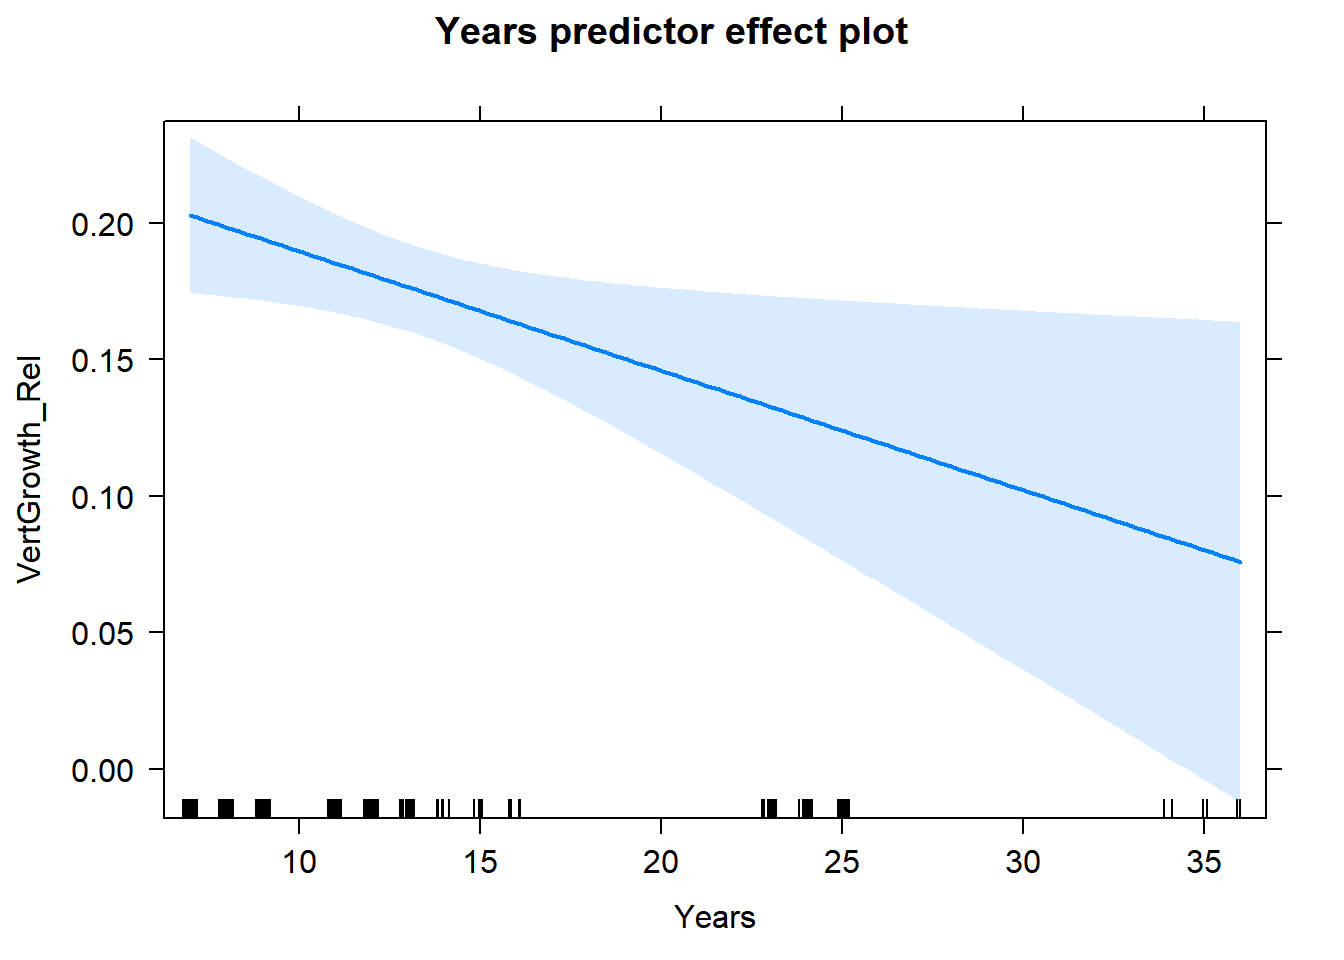
\includegraphics{simulations_files/figure-latex/unnamed-chunk-29-1.pdf}

\begin{Shaded}
\begin{Highlighting}[]
\KeywordTok{ggsave}\NormalTok{(}\DataTypeTok{file =} \StringTok{"../../results/figures/sim_1000_hts.png"}\NormalTok{, }\DataTypeTok{width =} \DecValTok{6}\NormalTok{, }\DataTypeTok{height =}\DecValTok{4}\NormalTok{, }\DataTypeTok{dpi =} \DecValTok{400}\NormalTok{)}
\end{Highlighting}
\end{Shaded}

\begin{verbatim}
## `geom_smooth()` using method = 'gam' and formula 'y ~ s(x, bs = "cs")'
\end{verbatim}

\subsection{Height by year and
species}\label{height-by-year-and-species}

\subsubsection{Shrub growth patterns}\label{shrub-growth-patterns-1}

\begin{Shaded}
\begin{Highlighting}[]
\KeywordTok{ggplot}\NormalTok{(dfsimallreps_summary }\OperatorTok\StringTok{ }\KeywordTok{filter}\NormalTok{(Species }\OperatorTok{==}\StringTok{ "ABCO"}\NormalTok{))}\OperatorTok{+}
\StringTok{  }\KeywordTok{geom_line}\NormalTok{(}\KeywordTok{aes}\NormalTok{(}\DataTypeTok{x =}\NormalTok{ Years, }\DataTypeTok{y =}\NormalTok{ Ht1.}\DecValTok{3}\NormalTok{, }\DataTypeTok{col =}\NormalTok{ ShrubSpp03, }\DataTypeTok{group =}\NormalTok{ Sdlg))}\OperatorTok{+}
\StringTok{  }\KeywordTok{theme_bw}\NormalTok{()}
\end{Highlighting}
\end{Shaded}

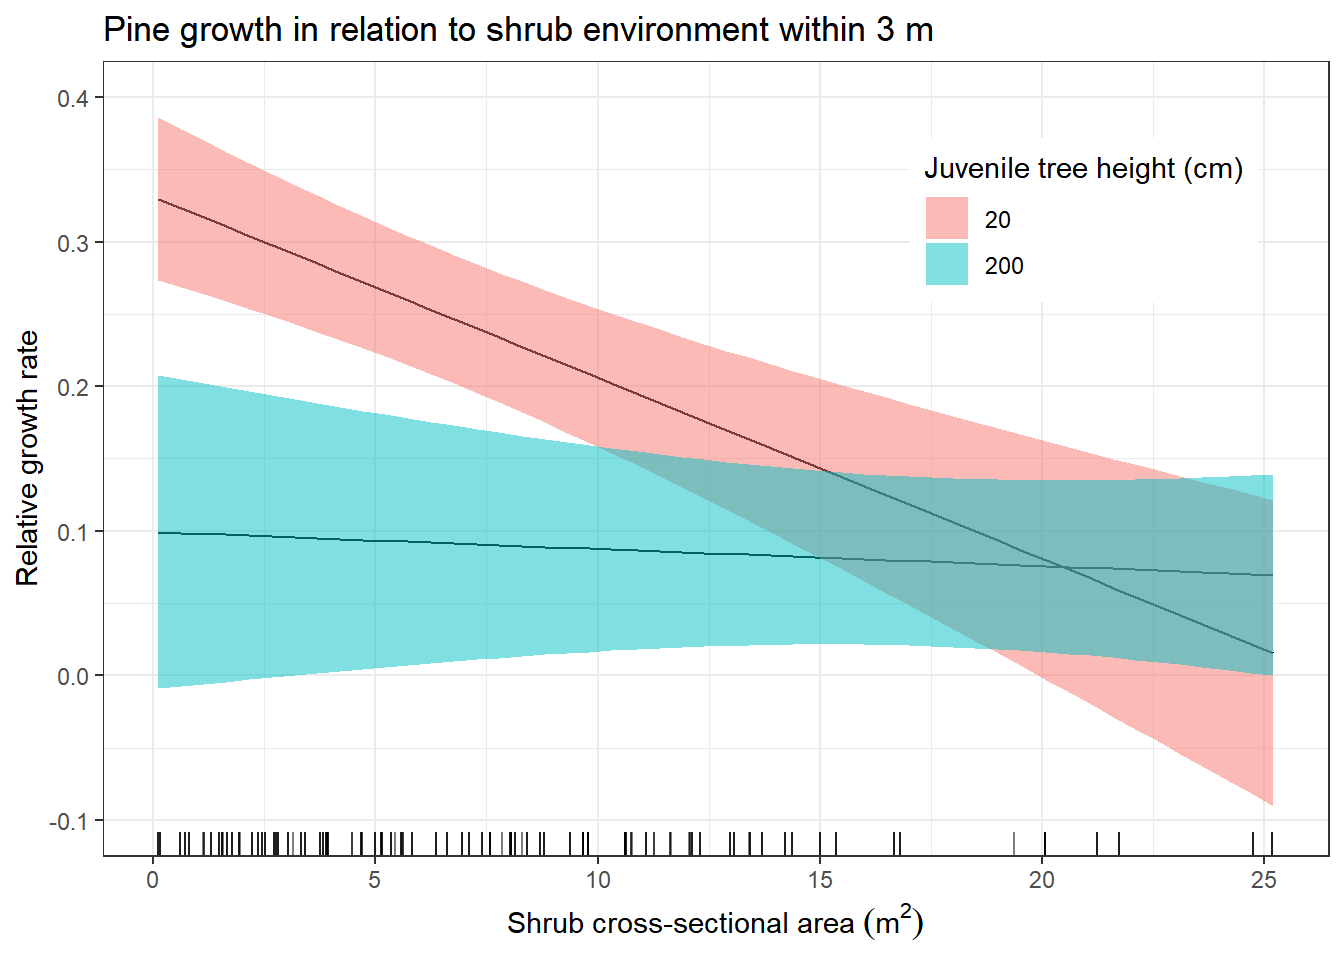
\includegraphics{simulations_files/figure-latex/unnamed-chunk-30-1.pdf}

\begin{Shaded}
\begin{Highlighting}[]
\KeywordTok{ggplot}\NormalTok{(dfsimallreps_summary }\OperatorTok\StringTok{ }\KeywordTok{filter}\NormalTok{(Species }\OperatorTok{==}\StringTok{ "PIPO"}\NormalTok{))}\OperatorTok{+}
\StringTok{  }\KeywordTok{geom_line}\NormalTok{(}\KeywordTok{aes}\NormalTok{(}\DataTypeTok{x =}\NormalTok{ Years, }\DataTypeTok{y =}\NormalTok{ Ht1.}\DecValTok{3}\NormalTok{, }\DataTypeTok{col =}\NormalTok{ ShrubSpp03, }\DataTypeTok{group =}\NormalTok{ Sdlg))}\OperatorTok{+}
\StringTok{  }\KeywordTok{theme_bw}\NormalTok{()}
\end{Highlighting}
\end{Shaded}

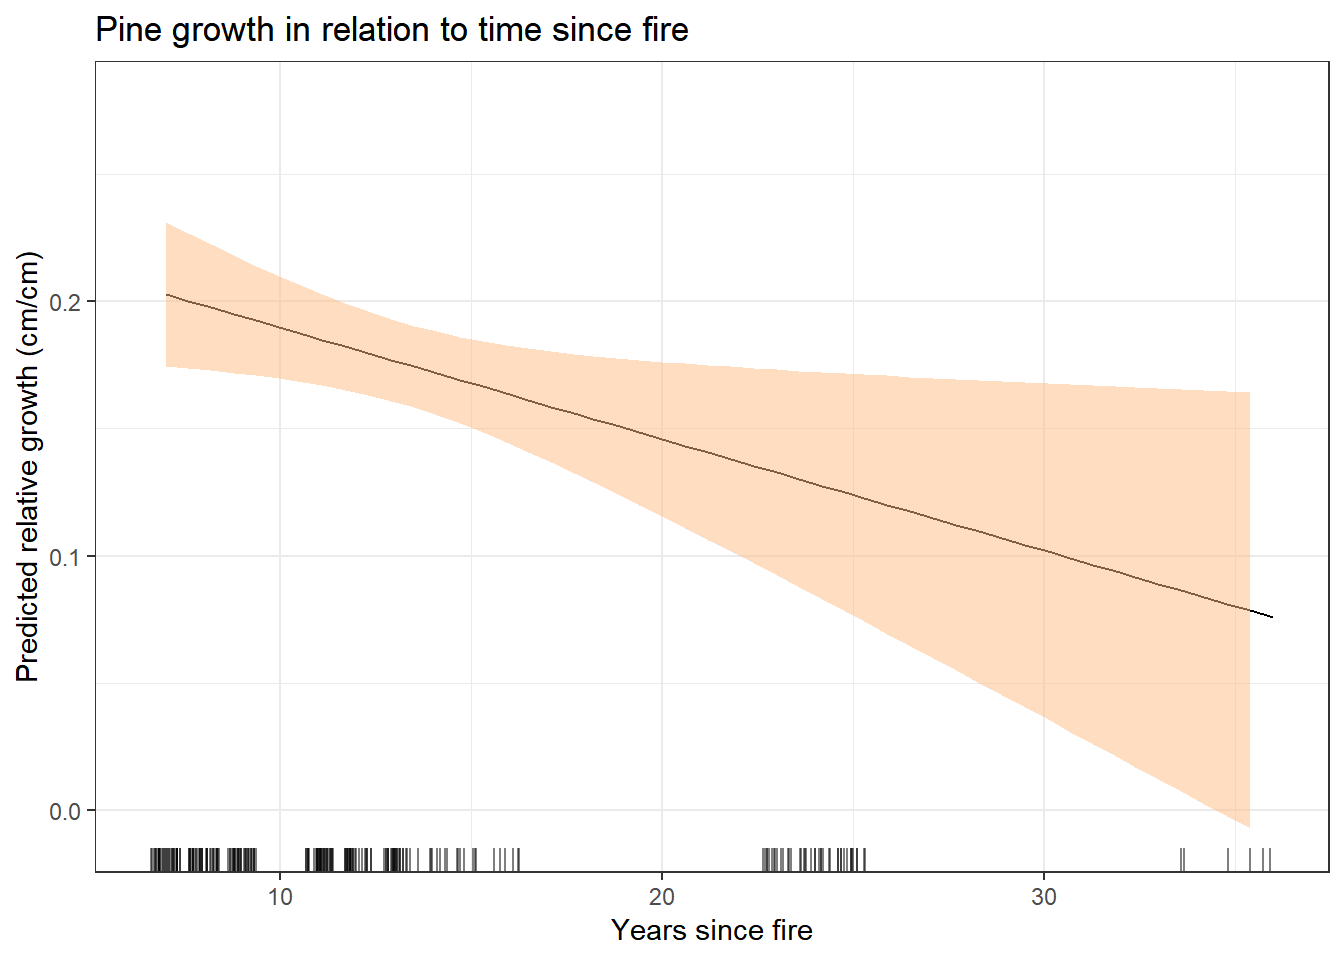
\includegraphics{simulations_files/figure-latex/unnamed-chunk-31-1.pdf}

\subsubsection{Diameter growth
patterns}\label{diameter-growth-patterns-1}

\begin{Shaded}
\begin{Highlighting}[]
\KeywordTok{ggplot}\NormalTok{(dfsimallreps_summary, }\KeywordTok{aes}\NormalTok{(}\DataTypeTok{x =}\NormalTok{ Years, }\DataTypeTok{y =}\NormalTok{ dia.cm, }\DataTypeTok{col =}\NormalTok{ Species, }\DataTypeTok{group =}\NormalTok{ Sdlg))}\OperatorTok{+}
\StringTok{  }\KeywordTok{geom_line}\NormalTok{(}\DataTypeTok{alpha =}\NormalTok{ .}\DecValTok{3}\NormalTok{)}\OperatorTok{+}
\StringTok{  }\KeywordTok{theme_bw}\NormalTok{()}\OperatorTok{+}
\StringTok{  }\KeywordTok{geom_smooth}\NormalTok{(}\KeywordTok{aes}\NormalTok{(}\DataTypeTok{x =}\NormalTok{ Years, }\DataTypeTok{y =}\NormalTok{ dia.cm, }\DataTypeTok{col =}\NormalTok{ Species, }\DataTypeTok{group =}\NormalTok{ Species))}
\end{Highlighting}
\end{Shaded}

\begin{verbatim}
## `geom_smooth()` using method = 'gam' and formula 'y ~ s(x, bs = "cs")'
\end{verbatim}

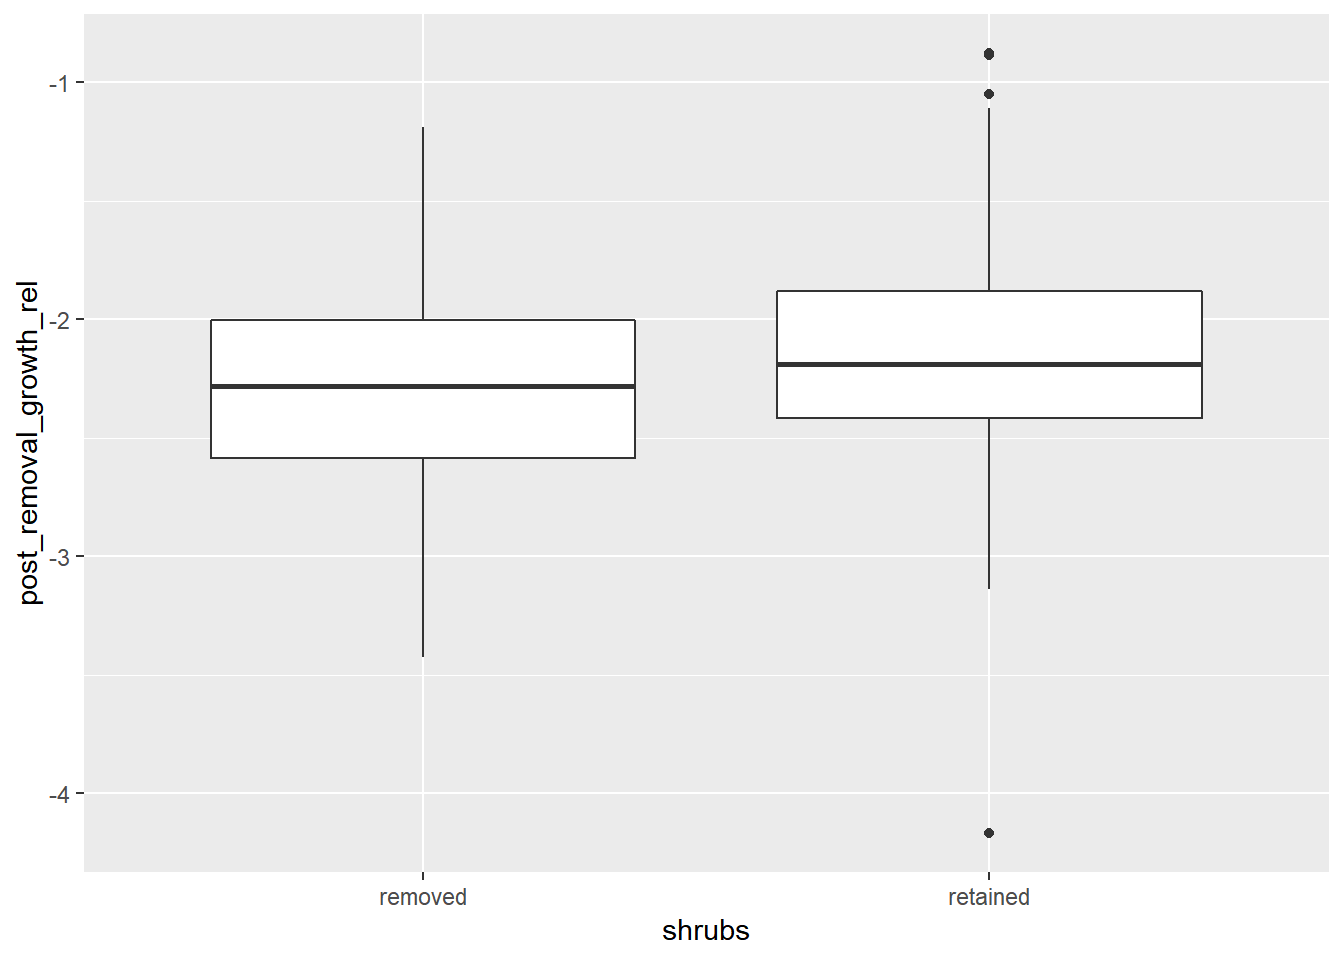
\includegraphics{simulations_files/figure-latex/unnamed-chunk-32-1.pdf}

\subsubsection{Height growth patterns}\label{height-growth-patterns-1}

\begin{Shaded}
\begin{Highlighting}[]
\KeywordTok{ggplot}\NormalTok{(dfsimallreps_summary, }\KeywordTok{aes}\NormalTok{(}\DataTypeTok{x =}\NormalTok{ Years, }\DataTypeTok{y =}\NormalTok{ Ht_cm1, }\DataTypeTok{col =}\NormalTok{ Species, }\DataTypeTok{group =}\NormalTok{ Sdlg))}\OperatorTok{+}
\StringTok{  }\KeywordTok{geom_line}\NormalTok{(}\DataTypeTok{alpha =}\NormalTok{ .}\DecValTok{3}\NormalTok{)}\OperatorTok{+}
\StringTok{  }\KeywordTok{theme_bw}\NormalTok{()}\OperatorTok{+}
\StringTok{  }\KeywordTok{geom_smooth}\NormalTok{(}\KeywordTok{aes}\NormalTok{(}\DataTypeTok{x =}\NormalTok{ Years, }\DataTypeTok{y =}\NormalTok{ Ht_cm1, }\DataTypeTok{col =}\NormalTok{ Species, }\DataTypeTok{group =}\NormalTok{ Species))}
\end{Highlighting}
\end{Shaded}

\begin{verbatim}
## `geom_smooth()` using method = 'gam' and formula 'y ~ s(x, bs = "cs")'
\end{verbatim}

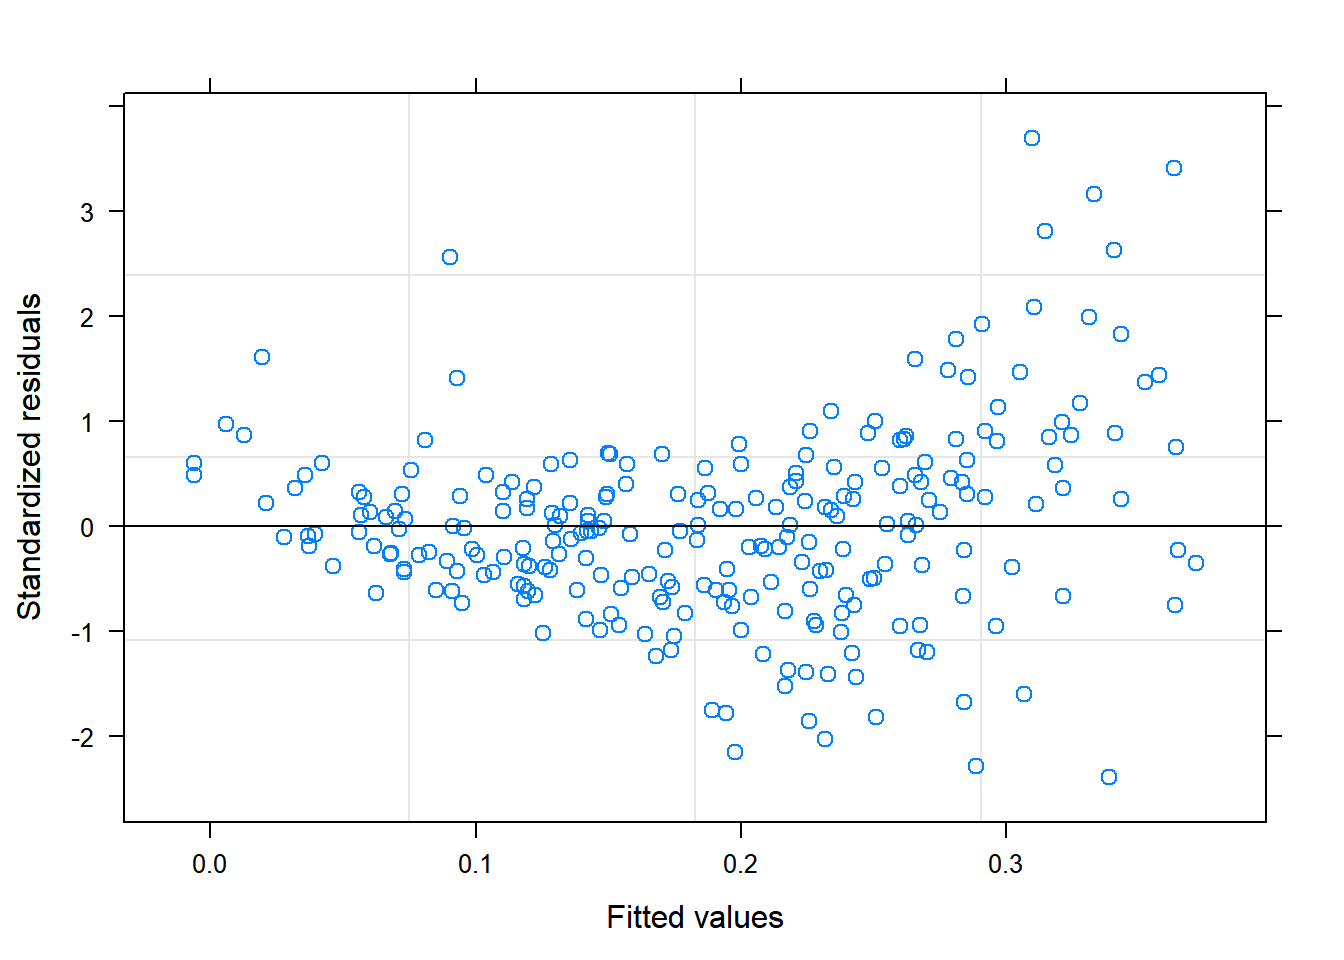
\includegraphics{simulations_files/figure-latex/unnamed-chunk-33-1.pdf}

\subsubsection{Diameter::Height growth
patterns}\label{diameterheight-growth-patterns-1}

\begin{Shaded}
\begin{Highlighting}[]
\KeywordTok{ggplot}\NormalTok{(dfsimallreps_summary, }\KeywordTok{aes}\NormalTok{(}\DataTypeTok{x =}\NormalTok{ Years, }\DataTypeTok{y =}\NormalTok{ dia.cm}\OperatorTok{/}\NormalTok{Ht_cm1, }\DataTypeTok{col =}\NormalTok{ Species, }\DataTypeTok{group =}\NormalTok{ Sdlg))}\OperatorTok{+}
\StringTok{  }\KeywordTok{geom_line}\NormalTok{(}\DataTypeTok{alpha =}\NormalTok{ .}\DecValTok{3}\NormalTok{)}\OperatorTok{+}
\StringTok{  }\KeywordTok{theme_bw}\NormalTok{()}\OperatorTok{+}
\StringTok{  }\KeywordTok{geom_smooth}\NormalTok{(}\KeywordTok{aes}\NormalTok{(}\DataTypeTok{x =}\NormalTok{ Years, }\DataTypeTok{y =}\NormalTok{ dia.cm}\OperatorTok{/}\NormalTok{Ht_cm1, }\DataTypeTok{col =}\NormalTok{ Species, }\DataTypeTok{group =}\NormalTok{ Species))}
\end{Highlighting}
\end{Shaded}

\begin{verbatim}
## `geom_smooth()` using method = 'gam' and formula 'y ~ s(x, bs = "cs")'
\end{verbatim}

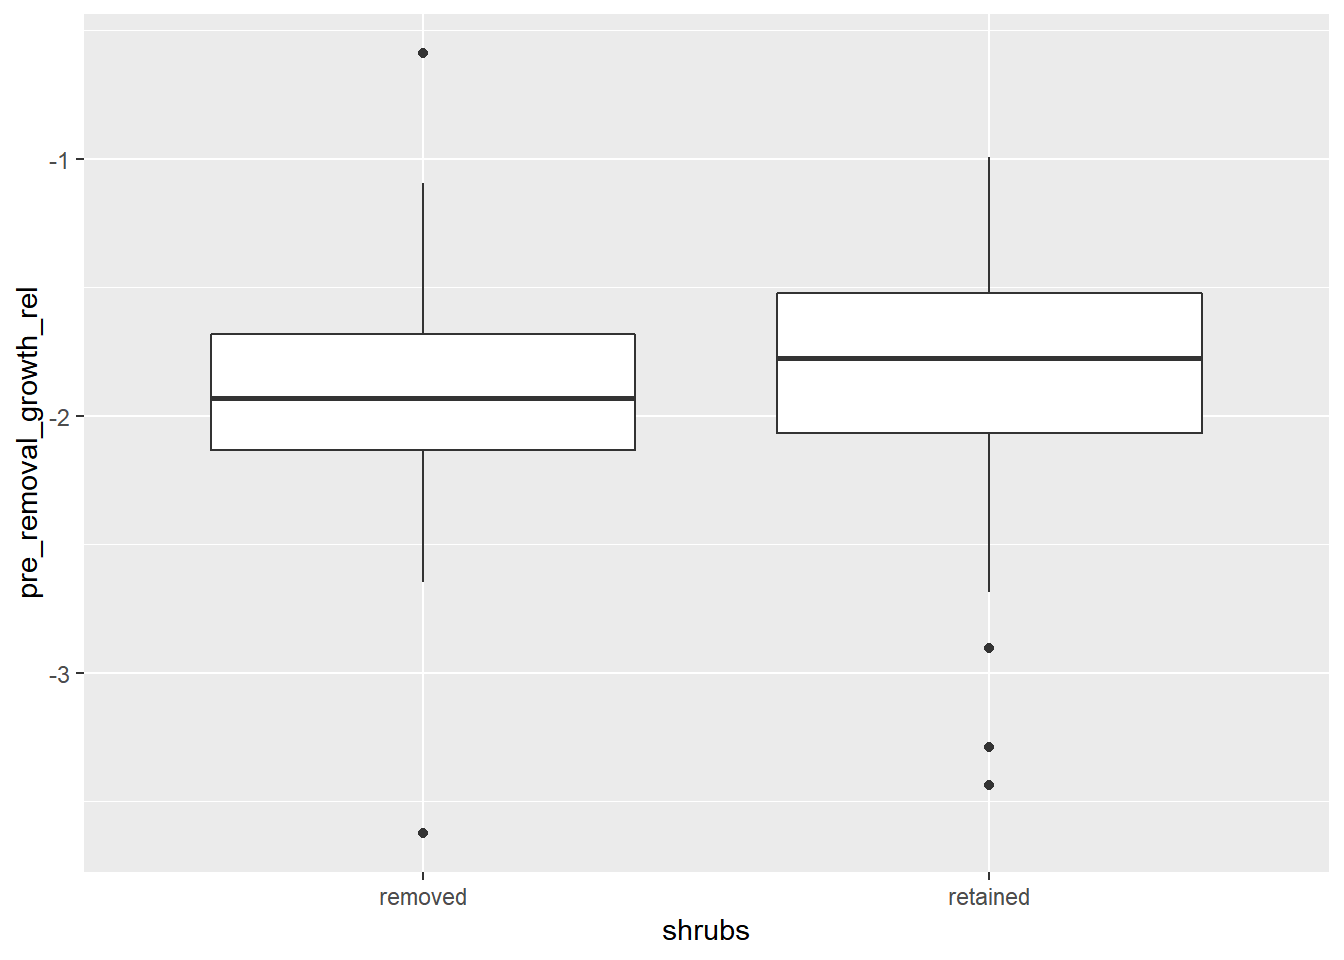
\includegraphics{simulations_files/figure-latex/unnamed-chunk-34-1.pdf}

\subsubsection{Diameter:height}\label{diameterheight-1}

\begin{Shaded}
\begin{Highlighting}[]
\KeywordTok{ggplot}\NormalTok{(dfsimallreps_summary }\OperatorTok\StringTok{ }\KeywordTok{filter}\NormalTok{(Years}\OperatorTok{==}\DecValTok{10}\NormalTok{))}\OperatorTok{+}
\StringTok{  }\KeywordTok{geom_histogram}\NormalTok{(}\KeywordTok{aes}\NormalTok{(dia.cm}\OperatorTok{/}\NormalTok{Ht_cm1, }\DataTypeTok{bins =} \DecValTok{20}\NormalTok{))}
\end{Highlighting}
\end{Shaded}

\begin{verbatim}
## Warning: Ignoring unknown aesthetics: bins
\end{verbatim}

\begin{verbatim}
## `stat_bin()` using `bins = 30`. Pick better value with `binwidth`.
\end{verbatim}

\includegraphics{simulations_files/figure-latex/unnamed-chunk-35-1.pdf}

\begin{Shaded}
\begin{Highlighting}[]
\KeywordTok{ggplot}\NormalTok{(dfsimallreps_summary }\OperatorTok\StringTok{ }\KeywordTok{filter}\NormalTok{(Years}\OperatorTok{==}\DecValTok{20}\NormalTok{))}\OperatorTok{+}
\StringTok{  }\KeywordTok{geom_histogram}\NormalTok{(}\KeywordTok{aes}\NormalTok{(dia.cm}\OperatorTok{/}\NormalTok{Ht_cm1, }\DataTypeTok{bins =} \DecValTok{20}\NormalTok{))}
\end{Highlighting}
\end{Shaded}

\begin{verbatim}
## Warning: Ignoring unknown aesthetics: bins
\end{verbatim}

\begin{verbatim}
## `stat_bin()` using `bins = 30`. Pick better value with `binwidth`.
\end{verbatim}

\includegraphics{simulations_files/figure-latex/unnamed-chunk-35-2.pdf}

\subsubsection{Diameter and height
boxplots}\label{diameter-and-height-boxplots-1}

\begin{Shaded}
\begin{Highlighting}[]
\KeywordTok{ggplot}\NormalTok{(dfsimallreps_summary)}\OperatorTok{+}
\StringTok{  }\KeywordTok{geom_boxplot}\NormalTok{(}\KeywordTok{aes}\NormalTok{(}\DataTypeTok{x =} \KeywordTok{as.factor}\NormalTok{(Years), }\DataTypeTok{y =}\NormalTok{ dia.cm, }\DataTypeTok{fill =}\NormalTok{ Species))}\OperatorTok{+}
\StringTok{  }\KeywordTok{theme_minimal}\NormalTok{()}\OperatorTok{+}
\StringTok{  }\KeywordTok{xlab}\NormalTok{(}\StringTok{"Years"}\NormalTok{)}\OperatorTok{+}
\StringTok{  }\KeywordTok{ylab}\NormalTok{(}\StringTok{"Diameter (cm)"}\NormalTok{)}\OperatorTok{+}
\StringTok{  }\KeywordTok{theme}\NormalTok{(}\DataTypeTok{text =} \KeywordTok{element_text}\NormalTok{(}\DataTypeTok{size =} \DecValTok{20}\NormalTok{))}\OperatorTok{+}
\StringTok{  }\KeywordTok{scale_x_discrete}\NormalTok{(}\DataTypeTok{name =} \StringTok{"Years since fire"}\NormalTok{, }\DataTypeTok{breaks =} \KeywordTok{c}\NormalTok{(}\StringTok{"10"}\NormalTok{, }\StringTok{"15"}\NormalTok{, }\StringTok{"20"}\NormalTok{, }\StringTok{"25"}\NormalTok{))}
\end{Highlighting}
\end{Shaded}

\includegraphics{simulations_files/figure-latex/unnamed-chunk-36-1.pdf}

\begin{Shaded}
\begin{Highlighting}[]
\KeywordTok{ggplot}\NormalTok{(dfsimall)}\OperatorTok{+}
\StringTok{  }\KeywordTok{geom_boxplot}\NormalTok{(}\KeywordTok{aes}\NormalTok{(}\DataTypeTok{x =} \KeywordTok{as.factor}\NormalTok{(Years), }\DataTypeTok{y =}\NormalTok{ Ht_cm1, }\DataTypeTok{fill =}\NormalTok{ Species))}\OperatorTok{+}
\StringTok{  }\KeywordTok{theme_minimal}\NormalTok{()}\OperatorTok{+}
\StringTok{  }\KeywordTok{xlab}\NormalTok{(}\StringTok{"Years"}\NormalTok{)}\OperatorTok{+}
\StringTok{  }\KeywordTok{ylab}\NormalTok{(}\StringTok{"Height (cm)"}\NormalTok{)}\OperatorTok{+}
\StringTok{  }\KeywordTok{theme}\NormalTok{(}\DataTypeTok{text =} \KeywordTok{element_text}\NormalTok{(}\DataTypeTok{size =} \DecValTok{20}\NormalTok{))}\OperatorTok{+}
\StringTok{  }\KeywordTok{scale_x_discrete}\NormalTok{(}\DataTypeTok{name =} \StringTok{"Years since fire"}\NormalTok{, }\DataTypeTok{breaks =} \KeywordTok{c}\NormalTok{(}\StringTok{"10"}\NormalTok{, }\StringTok{"15"}\NormalTok{, }\StringTok{"20"}\NormalTok{, }\StringTok{"25"}\NormalTok{))}
\end{Highlighting}
\end{Shaded}

\includegraphics{simulations_files/figure-latex/unnamed-chunk-37-1.pdf}

\subsection{Counts by year}\label{counts-by-year}

\begin{Shaded}
\begin{Highlighting}[]
\NormalTok{dfsimallreps_summary <-}\StringTok{ }\NormalTok{dfsimallreps }\OperatorTok\StringTok{ }
\StringTok{  }\KeywordTok{ungroup}\NormalTok{() }\OperatorTok\StringTok{ }
\StringTok{  }\KeywordTok{group_by}\NormalTok{(rep, Years, Species) }\OperatorTok\StringTok{ }
\StringTok{  }\KeywordTok{mutate}\NormalTok{(}\DataTypeTok{count =} \KeywordTok{n}\NormalTok{()) }\OperatorTok\StringTok{ }
\StringTok{  }\KeywordTok{mutate}\NormalTok{(}\DataTypeTok{count =} \KeywordTok{as.numeric}\NormalTok{(count))}
\end{Highlighting}
\end{Shaded}

\begin{Shaded}
\begin{Highlighting}[]
\KeywordTok{ggplot}\NormalTok{(dfsimallreps_summary, }\KeywordTok{aes}\NormalTok{(}\DataTypeTok{x =} \KeywordTok{as.factor}\NormalTok{(Years), }\DataTypeTok{y =}\NormalTok{ count, }\DataTypeTok{fill =}\NormalTok{ Species, }\DataTypeTok{col =}\NormalTok{ Species))}\OperatorTok{+}
\StringTok{  }\KeywordTok{geom_boxplot}\NormalTok{(}\DataTypeTok{alpha =}\NormalTok{ .}\DecValTok{2}\NormalTok{, }\DataTypeTok{outlier.alpha =}\NormalTok{ .}\DecValTok{02}\NormalTok{)}\OperatorTok{+}
\StringTok{  }\KeywordTok{geom_smooth}\NormalTok{(}\KeywordTok{aes}\NormalTok{(}\DataTypeTok{x =} \KeywordTok{as.factor}\NormalTok{(Years), }\DataTypeTok{y =}\NormalTok{ count, }\DataTypeTok{fill =}\NormalTok{ Species, }\DataTypeTok{col =}\NormalTok{ Species), }\DataTypeTok{size =} \DecValTok{1}\NormalTok{)}\OperatorTok{+}
\StringTok{  }\KeywordTok{ggtitle}\NormalTok{(}\StringTok{"Results for 1000 simulations"}\NormalTok{)}\OperatorTok{+}
\StringTok{  }\KeywordTok{xlab}\NormalTok{(}\StringTok{"Years since fire"}\NormalTok{)}\OperatorTok{+}
\StringTok{  }\KeywordTok{ylab}\NormalTok{(}\StringTok{"Tree count"}\NormalTok{)}\OperatorTok{+}
\StringTok{  }\KeywordTok{theme_bw}\NormalTok{()}\OperatorTok{+}
\StringTok{  }\KeywordTok{scale_color_manual}\NormalTok{(}\DataTypeTok{values =} \KeywordTok{c}\NormalTok{(}\StringTok{"#899DA4"}\NormalTok{, }\StringTok{"#9A8822"}\NormalTok{), }\DataTypeTok{labels =} \KeywordTok{c}\NormalTok{(}\StringTok{"Fir"}\NormalTok{, }\StringTok{"Pine"}\NormalTok{))}\OperatorTok{+}
\StringTok{  }\KeywordTok{scale_fill_manual}\NormalTok{(}\DataTypeTok{values =} \KeywordTok{c}\NormalTok{(}\StringTok{"#899DA4"}\NormalTok{, }\StringTok{"#9A8822"}\NormalTok{), }\DataTypeTok{labels =} \KeywordTok{c}\NormalTok{(}\StringTok{"Fir"}\NormalTok{, }\StringTok{"Pine"}\NormalTok{))}\OperatorTok{+}
\StringTok{  }\KeywordTok{theme}\NormalTok{(}\DataTypeTok{text =} \KeywordTok{element_text}\NormalTok{(}\DataTypeTok{size =} \DecValTok{16}\NormalTok{), }
        \DataTypeTok{panel.grid.minor.x =} \KeywordTok{element_blank}\NormalTok{(),}
        \DataTypeTok{panel.grid.major.x =} \KeywordTok{element_blank}\NormalTok{(),}
        \DataTypeTok{axis.text.x =} \KeywordTok{element_text}\NormalTok{(}\DataTypeTok{size =} \DecValTok{8}\NormalTok{))}
\end{Highlighting}
\end{Shaded}

\begin{verbatim}
## `geom_smooth()` using method = 'gam' and formula 'y ~ s(x, bs = "cs")'
\end{verbatim}

\includegraphics{simulations_files/figure-latex/unnamed-chunk-39-1.pdf}

\begin{Shaded}
\begin{Highlighting}[]
\KeywordTok{ggsave}\NormalTok{(}\DataTypeTok{file =} \StringTok{"../../results/figures/sim_1000_count.png"}\NormalTok{, }\DataTypeTok{width =} \DecValTok{6}\NormalTok{, }\DataTypeTok{height =} \DecValTok{4}\NormalTok{, }\DataTypeTok{dpi =} \DecValTok{400}\NormalTok{)}
\end{Highlighting}
\end{Shaded}

\begin{verbatim}
## `geom_smooth()` using method = 'gam' and formula 'y ~ s(x, bs = "cs")'
\end{verbatim}

\subsection{Shrub height by year}\label{shrub-height-by-year}

\begin{Shaded}
\begin{Highlighting}[]
\NormalTok{dfsimallreps_summary <-}\StringTok{ }\NormalTok{dfsimallreps }\OperatorTok\StringTok{ }
\StringTok{  }\KeywordTok{ungroup}\NormalTok{() }\OperatorTok\StringTok{ }
\StringTok{  }\KeywordTok{group_by}\NormalTok{(rep, Years, Ht1.}\DecValTok{3}\NormalTok{, ShrubSpp03) }\OperatorTok\StringTok{ }
\StringTok{  }\KeywordTok{mutate}\NormalTok{(}\DataTypeTok{mean_shrub_ht =} \KeywordTok{mean}\NormalTok{(Ht1.}\DecValTok{3}\NormalTok{))}
\end{Highlighting}
\end{Shaded}

\begin{Shaded}
\begin{Highlighting}[]
\KeywordTok{ggplot}\NormalTok{(dfsimallreps_summary, }\KeywordTok{aes}\NormalTok{(}\DataTypeTok{x =}\NormalTok{ Years, }\DataTypeTok{y =}\NormalTok{ mean_shrub_ht, }\DataTypeTok{group =}\NormalTok{ ShrubSpp03, }\DataTypeTok{col =}\NormalTok{ ShrubSpp03))}\OperatorTok{+}
\StringTok{  }\KeywordTok{geom_line}\NormalTok{(}\KeywordTok{aes}\NormalTok{(}\DataTypeTok{group =}\NormalTok{ Sdlg), }\DataTypeTok{alpha =}\NormalTok{ .}\DecValTok{2}\NormalTok{)}\OperatorTok{+}
\StringTok{  }\KeywordTok{geom_smooth}\NormalTok{()}\OperatorTok{+}
\StringTok{  }\KeywordTok{ggtitle}\NormalTok{(}\StringTok{"Results for 1000 simulations"}\NormalTok{)}\OperatorTok{+}
\StringTok{  }\KeywordTok{xlab}\NormalTok{(}\StringTok{"Years since fire"}\NormalTok{)}\OperatorTok{+}
\StringTok{  }\KeywordTok{ylab}\NormalTok{(}\StringTok{"Shrub height"}\NormalTok{)}\OperatorTok{+}
\StringTok{  }\KeywordTok{theme_bw}\NormalTok{()}
\end{Highlighting}
\end{Shaded}

\begin{verbatim}
## `geom_smooth()` using method = 'gam' and formula 'y ~ s(x, bs = "cs")'
\end{verbatim}

\includegraphics{simulations_files/figure-latex/unnamed-chunk-41-1.pdf}

\begin{Shaded}
\begin{Highlighting}[]
\KeywordTok{print}\NormalTok{(}\KeywordTok{Sys.time}\NormalTok{() }\OperatorTok{-}\StringTok{ }\NormalTok{strt)}
\end{Highlighting}
\end{Shaded}

\begin{verbatim}
## Time difference of 1.767178 hours
\end{verbatim}

\section{Seedling height by shrub species and
year}\label{seedling-height-by-shrub-species-and-year}

\begin{Shaded}
\begin{Highlighting}[]
\NormalTok{dfsimallreps_summary <-}\StringTok{ }\NormalTok{dfsimallreps }\OperatorTok\StringTok{ }
\StringTok{  }\KeywordTok{ungroup}\NormalTok{() }\OperatorTok\StringTok{ }
\StringTok{  }\KeywordTok{group_by}\NormalTok{(Species, rep, Years, Ht_cm1, ShrubSpp03) }\OperatorTok\StringTok{ }
\StringTok{  }\KeywordTok{mutate}\NormalTok{(}\DataTypeTok{mean_ht =} \KeywordTok{mean}\NormalTok{(Ht_cm1))}
\end{Highlighting}
\end{Shaded}

\begin{Shaded}
\begin{Highlighting}[]
\KeywordTok{ggplot}\NormalTok{(dfsimallreps_summary, }\KeywordTok{aes}\NormalTok{(}\DataTypeTok{x =}\NormalTok{ Years, }\DataTypeTok{y =}\NormalTok{ Ht_cm1, }\DataTypeTok{group =}\NormalTok{ ShrubSpp03, }\DataTypeTok{col =}\NormalTok{ ShrubSpp03, }\DataTypeTok{symbol =}\NormalTok{ Species))}\OperatorTok{+}
\StringTok{  }\KeywordTok{geom_line}\NormalTok{(}\KeywordTok{aes}\NormalTok{(}\DataTypeTok{group =}\NormalTok{ Sdlg), }\DataTypeTok{alpha =}\NormalTok{ .}\DecValTok{2}\NormalTok{)}\OperatorTok{+}
\StringTok{  }\KeywordTok{geom_smooth}\NormalTok{()}\OperatorTok{+}
\StringTok{  }\KeywordTok{ggtitle}\NormalTok{(}\StringTok{"Results for 1000 simulations"}\NormalTok{)}\OperatorTok{+}
\StringTok{  }\KeywordTok{xlab}\NormalTok{(}\StringTok{"Years since fire"}\NormalTok{)}\OperatorTok{+}
\StringTok{  }\KeywordTok{ylab}\NormalTok{(}\StringTok{"Focal tree height"}\NormalTok{)}\OperatorTok{+}
\StringTok{  }\KeywordTok{theme_bw}\NormalTok{()}
\end{Highlighting}
\end{Shaded}

\begin{verbatim}
## `geom_smooth()` using method = 'gam' and formula 'y ~ s(x, bs = "cs")'
\end{verbatim}

\includegraphics{simulations_files/figure-latex/unnamed-chunk-44-1.pdf}

\section{Next steps to improve the
model}\label{next-steps-to-improve-the-model}

\begin{enumerate}
\def\labelenumi{\arabic{enumi}.}
\tightlist
\item
  Use Kristen's data or Hugh's data for initial conditions
\item
  Improve dispersal kernel based on Kristen/Hugh's data
\item
  Improve shrub growth based on data - DONE
\item
  Include residual surviving trees and their seed dispersal
\item
  Include seed dispersal of post-fire regen once it reaches reproductive
  age
\item
  Add customization of patch size and shape
\item
  Add customization of whether the weather conditions reflect those of
  2015, 2016, or 2017
\item
  Change sapling growth equations once they emerge from the shrub canopy
\end{enumerate}

For next week: - Improve shrub growth based on data - DONE - display
dominant shrub species - make the shrub grid dependent upon surrounding
cells so it's not so checkerboard - DONE - Update display of shrub
competition after simulation years - what does shrub competition mean
for new recruitment? - ``emergent year'' = when 50\% of trees are above
shrub canopy - apply to King, American River Complex, rest of the fires
I measured - switch diameter equation to be from dendro work

Other notes: - maybe submit to American Naturalist - Global Change
Biology - mixing up the years - no overstory reproduction for now


\end{document}
